% ОБЯЗАТЕЛЬНО ИМЕННО ТАКОЙ documentclass!
% (Основной кегль = 14pt, поэтому необходим extsizes)
% Формат, разумеется, А4
% article потому что стандарт не подразумевает разделов
% Глава = section, Параграф = subsection
% (понятия "глава" и "параграф" из документа, описывающего диплом)
\documentclass[a4paper,article,14pt]{extarticle}

% Подключаем главный пакет со всем необходимым
\usepackage{spbudiploma}

% Пакеты по желанию (самые распространенные)
% Хитрые мат. символы
\usepackage{euscript}
% Таблицы
\usepackage{longtable}
\usepackage{makecell}
% Картинки (можно встявлять даже pdf)
\usepackage[pdftex]{graphicx}

\usepackage{amsthm,amssymb,amsmath}
\usepackage{mathtools}
\usepackage{textcomp}

\usepackage{subcaption}
\usepackage{stmaryrd}
\usepackage{mathpartir}
\usepackage{thm-restate}
\usepackage{thmtools,thm-restate}
\usepackage{xspace}
\usepackage{multicol}
\usepackage{xifthen}

\usepackage{tikz}
\usetikzlibrary{chains}             
\usetikzlibrary{shapes.geometric}   
\usetikzlibrary{shapes.symbols}     
\usetikzlibrary{arrows}             
\usetikzlibrary{fit} 
\usetikzlibrary{backgrounds} 
\usetikzlibrary{positioning} 
\usetikzlibrary{calc} 
\usetikzlibrary{patterns} 
\usetikzlibrary{snakes} 

\usepackage{bussproofs}
\EnableBpAbbreviations

\usepackage{cleveref}

%%%%%%%%%%%%%%%%%%%%%%%%%%%%%%%%%%%%%%%%%%%%%%%%%%%%%%%%%%%%%%%%%%%%%%%%%%%%%%%%
%%%%  Misc. Math  %%%%%%%%%%%%%%%%%%%%%%%%%%%%%%%%%%%%%%%%%%%%%%%%%%%%%%%%%%%%%%
%%%%%%%%%%%%%%%%%%%%%%%%%%%%%%%%%%%%%%%%%%%%%%%%%%%%%%%%%%%%%%%%%%%%%%%%%%%%%%%%

% set notation
\newcommand{\set}[1]{\{#1\}}

% sequence notation
\newcommand{\seq}[1]{[{#1}]}

% tuple with angle brackets
\newcommand{\tup}[1]{\langle #1 \rangle}

% first and second components of a pair
\newcommand{\fst}[1]{\mathit{fst}(#1)}
\newcommand{\snd}[1]{\mathit{snd}(#1)}

% semantics brackets
\newcommand{\sem}[1]{\llbracket #1 \rrbracket}

% equality by definition
\newcommand{\defeq}{\triangleq}

% function arrow
\newcommand{\fun}{\rightarrow}

% partial function arrow
\newcommand{\pfun}{\rightharpoonup}

% shorter subset notation
\newcommand{\suq}{\subseteq}

% homomorphism arrow (TODO: change notations)
\newcommand{\homf}[1][{}]{\underset{#1}{\leadsto}}

% isomorphism 
\newcommand{\isof}[1][{}]{\underset{#1}\sim}

% power set
\newcommand{\pwset}[1]{\mathcal{P}(#1)}

% prefix/suffix 
\newcommand{\dwset}[1]{\overline{\lceil{#1}\rceil}}
\newcommand{\upset}[1]{\underline{\lfloor{#1}\rfloor}}

% strict prefix/suffix 
\newcommand{\dwsset}[1]{\lceil{#1}\rceil}
\newcommand{\upsset}[1]{\lfloor{#1}\rfloor}


% function-to-relation
\newcommand{\frel}[1]{#1^\uparrow}

% epsilon/empty 
\newcommand{\eps}{\epsilon}

% missing greek letters
\newcommand{\Tau}{\mathrm{T}}
\newcommand{\Ell}{\mathcal{L}}

% sequential composition (of relations)
\newcommand{\seqc}{\;}

% some math sets
\newcommand{\N}{{\mathbb{N}}}
\newcommand{\Z}{{\mathbb{Z}}}
\newcommand{\Q}{{\mathbb{Q}}}

% domain/codomain notation
\newcommand{\dom}[1]{\textit{dom}{({#1})}}
\newcommand{\cod}[1]{\textit{codom}{({#1})}}

% restriction
\newcommand{\rst}[1]{|_{#1}}

% length
\newcommand{\len}[1]{\mathsf{len}({#1})}

% cardinality
\newcommand{\card}[1]{|{#1}|}

%\newcommand{\implies}{{\Rightarrow}}
\renewcommand{\iff}{{\Longleftrightarrow}}

% finite subset
% \newcommand{\finsubseteq}{\underset{fin}{\subseteq}}
\newcommand{\finsubseteq}{{\subseteq}_{fin}}

% predecessor function
\newcommand{\pred}{\mathit{pred}}

% maps
\newcommand{\appmap}[2]{#1(#2)}
\newcommand{\updmap}[3]{#1[#2 \mapsto #3]}

% prefix order
\newcommand{\prefle}{\preccurlyeq}

%%%%%%%%%%%%%%%%%%%%%%%%%%%%%%%%%%%%%%%%%%%%%%%%%%%%%%%%%%%%%%%%%%%%%%%%%%%%%%%%
%%%%  LTS Defs  %%%%%%%%%%%%%%%%%%%%%%%%%%%%%%%%%%%%%%%%%%%%%%%%%%%%%%%%%%%%%%%%
%%%%%%%%%%%%%%%%%%%%%%%%%%%%%%%%%%%%%%%%%%%%%%%%%%%%%%%%%%%%%%%%%%%%%%%%%%%%%%%%

\newcommand{\LTS}{\Sigma}

% (labelled) transition 
\newcommand{\tr}[3][{}]{{#2}\xrightarrow[#1]{}{#3}}
\newcommand{\ltr}[4][{}]{{#3}\xrightarrow[#1]{#2}{#4}}

% to denote some state
\newcommand{\state}{\sigma}

% set of states
\newcommand{\State}{\mathbb{S}}

% function assigning initial states
\newcommand{\initst}{\iota}

% step tuple
\newcommand{\step}[3]{\tup{#2, #1, #3}}

% step tuple type
\newcommand{\Step}[2]{{#2 \times #1 \times #2}}

%%%%%%%%%%%%%%%%%%%%%%%%%%%%%%%%%%%%%%%%%%%%%%%%%%%%%%%%%%%%%%%%%%%%%%%%%%%%%%%%
%%%%  Pomsets and Event Struct. Defs  %%%%%%%%%%%%%%%%%%%%%%%%%%%%%%%%%%%%%%%%%%
%%%%%%%%%%%%%%%%%%%%%%%%%%%%%%%%%%%%%%%%%%%%%%%%%%%%%%%%%%%%%%%%%%%%%%%%%%%%%%%%

\newcommand{\lab}{\lambda}
\newcommand{\ca}{\leqslant}
\newcommand{\sca}{<}
\newcommand{\ica}{\lessdot}
\newcommand{\cf}{\#}
\newcommand{\icf}{\#^{\mu}}
\newcommand{\cons}{\mathcal{C}}
\newcommand{\gcf}{\mathbb{\#}}

% to denote some subset of events
\newcommand{\eset}{\mathcal{E}}

% set of all pomsets (generated by an alphabet)
\newcommand{\Pom}[1][{}]{%
  \textsc{Pom}\ifthenelse{\isempty{#1}}{}{(#1)}\xspace%
}

% set of all threaded pomsets (generated by an alphabet)
\newcommand{\ThrdPom}[1][{}]{%
  \textsc{ThrdPom}\ifthenelse{\isempty{#1}}{}{(#1)}\xspace%
}

% set of all deterministic pomsets (generated by an alphabet)
\newcommand{\DetPom}[1][{}]{%
  \textsc{DetPom}\ifthenelse{\isempty{#1}}{}{(#1)}\xspace%
}

% pomset language (generated by an alphabet)
\newcommand{\Pomlang}[1][{}]{%
  \textsc{Pomlang}\ifthenelse{\isempty{#1}}{}{(#1)}\xspace%
}

% set of all prime event structures (generated by an alphabet)
\newcommand{\PrimeES}[1][{}]{%
  \textsc{PES}\ifthenelse{\isempty{#1}}{}{(#1)}\xspace%
}

% set of all prime event structures (generated by an alphabet)
\newcommand{\ThrdPrimeES}[1][{}]{%
  \textsc{ThrdPES}\ifthenelse{\isempty{#1}}{}{(#1)}\xspace%
}

% pomset language of an event structure
\newcommand{\pomlang}[1]{\mathbf{Pom}(#1)\xspace}


\newcommand{\pomStep}[1]{\xhookrightarrow{#1}}
\newcommand{\esStep}[1]{\xrightarrow{#1}}

% step synchronization relation
\newcommand{\ssync}{\gg}
\newcommand{\posync}{\underset{\lPO}{\gg}}
\newcommand{\rfsync}{\underset{\lRF}{\gg}}

%%%%%%%%%%%%%%%%%%%%%%%%%%%%%%%%%%%%%%%%%%%%%%%%%%%%%%%%%%%%%%%%%%%%%%%%%%%%%%%%
%%%%  Weak Memory Defs  %%%%%%%%%%%%%%%%%%%%%%%%%%%%%%%%%%%%%%%%%%%%%%%%%%%%%%%%
%%%%%%%%%%%%%%%%%%%%%%%%%%%%%%%%%%%%%%%%%%%%%%%%%%%%%%%%%%%%%%%%%%%%%%%%%%%%%%%%

\newcommand{\Tid}{\mathsf{Tid}}
\newcommand{\Loc}{\mathsf{Loc}}
\newcommand{\Val}{\mathsf{Val}}
\newcommand{\Lab}{\mathsf{Lab}}
\newcommand{\Mod}{\mathsf{Mod}}

\newcommand{\isex}{{\mathtt{ex}}}
\newcommand{\isnotex}{{\operatorname{\mathtt{not-ex}}}}

\newcommand{\lR}{{\mathtt{R}}}
\newcommand{\lW}{{\mathtt{W}}}
\newcommand{\lF}{{\mathtt{F}}}
\newcommand{\lRex}{\lR_{\isex}}
\newcommand{\lWex}{\lW_{\isex}}
\newcommand{\lTS}{\mathtt{TS}}
\newcommand{\lTE}{\mathtt{TE}}

\newcommand{\wlab}[3]{{\lW}^{#1}({#2},{#3})}
\newcommand{\rlab}[3]{{\lR}^{#1}({#2},{#3})}
\newcommand{\flab}[1]{{\lF}^{#1}}
\newcommand{\ulab}[4]{{\lU}^{#1}({#2},{#3},{#4})}

\newcommand{\tslab}{{\lTS}}
\newcommand{\telab}{{\lTE}}

% initial value
\newcommand{\initval}{\bot}

\newcommand{\lE}{{\mathtt{E}}}
\newcommand{\Init}{\mathsf{Init}}

\newcommand{\lLAB}{{\mathtt{lab}}}
\newcommand{\lID}{{\mathtt{id}}}
\newcommand{\lTID}{{\mathtt{tid}}}
\newcommand{\lSN}{{\mathtt{sn}}}
\newcommand{\lTYP}{{\mathtt{typ}}}
\newcommand{\lLOC}{{\mathtt{loc}}}
\newcommand{\lMOD}{{\mathtt{mod}}}
\newcommand{\lVAL}{{\mathtt{val}}}
\newcommand{\lVALR}{{\mathtt{val_r}}}
\newcommand{\lVALW}{{\mathtt{val_w}}}
\newcommand{\lSTEP}{{\mathtt{st}}}

\newcommand{\lEQLAB}{=_{\lLAB}}
\newcommand{\lEQTID}{=_{\lTID}}
\newcommand{\lEQLOC}{=_{\lLOC}}
\newcommand{\lEQVAL}{=_{\lVAL}}

\colorlet{colorPO}{gray!60!black}
\colorlet{colorPPO}{magenta}
\colorlet{colorCF}{red!60!black}
\colorlet{colorECF}{red!60!black}
\colorlet{colorJF}{blue!60!black}
\colorlet{colorRF}{green!60!black}
\colorlet{colorEW}{brown}
\colorlet{colorMO}{orange}
\colorlet{colorFR}{purple}
\colorlet{colorECO}{orange!80!black}
\colorlet{colorSYN}{green!40!black}
\colorlet{colorHB}{blue}
\colorlet{colorPPO}{magenta}
\colorlet{colorRMW}{olive!70!black}
\colorlet{colorRS}{blue}
\colorlet{colorREL}{blue!70!black}
\colorlet{colorSC}{violet}
\colorlet{colorPSC}{violet}
\colorlet{colorWB}{orange!70!black}
\colorlet{colorSCB}{violet}
\colorlet{colorDETOUR}{teal}
\colorlet{colorDEPS}{violet}
\colorlet{colorFENCE}{olive}
\colorlet{colorCOV}{magenta!20}
\colorlet{colorISS}{blue!10!white}
\colorlet{colorVF}{purple!70!black}

\newcommand{\lPO}{{\color{colorPO}\mathtt{po}}}
\newcommand{\lPOimm}{{\color{colorPO}\mathtt{po_{imm}}}}
\newcommand{\lPPO}{{\color{colorPPO}\mathtt{ppo}}}
\newcommand{\lCF}{{\color{colorCF}\mathtt{cf}}}
\newcommand{\lCFimm}{{\color{colorCF}\mathtt{cf_{imm}}}}
\newcommand{\lECF}{{\color{colorECF}\mathtt{ecf}}}
\newcommand{\lJF}{{\color{colorJF} \mathtt{jf}}}
\newcommand{\lRF}{{\color{colorRF} \mathtt{rf}}}
\newcommand{\lPORF}{\lPO\lRF}
\newcommand{\lRMW}{{\color{colorRMW} \mathtt{rmw}}}
\newcommand{\lMO}{{\color{colorMO} \mathtt{mo}}}
\newcommand{\lEW}{{\color{colorEW} \mathtt{ew}}}
\newcommand{\lCO}{{\color{colorMO} \mathtt{co}}}
\newcommand{\lFR}{{\color{colorFR} \mathtt{fr}}}
\newcommand{\lECO}{{\color{colorECO} \mathtt{eco}}}
\newcommand{\lRS}{{\color{colorRS}\mathtt{rs}}}
\newcommand{\lREL}{{\color{colorREL}\mathtt{rel}}}
\newcommand{\lSW}{{\color{colorSYN}\mathtt{sw}}}
\newcommand{\lHB}{{\color{colorHB}\mathtt{hb}}}
\newcommand{\lBOB}{{\mathtt{bob}}}
\newcommand{\lSC}{{\color{colorSC}\mathtt{sc}}}

\tikzset{
   every path/.style={>=stealth},
   po/.style={->,color=colorPO,,shorten >=-0.5mm,shorten <=-0.5mm},
   por/.style={->,color=red,shorten >=-0.5mm,shorten <=-0.5mm},
   ppo/.style={->,color=colorPPO,,shorten >=-0.5mm,shorten <=-0.5mm},
   cf/.style={-,snake=zigzag,segment amplitude=1pt,segment length=3pt,colorCF},
   rmw/.style={->,color=colorRMW,,shorten >=-0.5mm,shorten <=-0.5mm},
   ca/.style={->,color=colorPO,thick,shorten >=-0.5mm,shorten <=-0.5mm},
   rf/.style={->,color=colorRF,dashed,,shorten >=-0.5mm,shorten <=-0.5mm},
   rfs/.style={->,color=colorRF,thick,dashed,,shorten >=-0.5mm,shorten <=-0.5mm},
   rb/.style={->,color=colorRB,thick,shorten >=-0.5mm,shorten <=-0.5mm},
   cc/.style={->,color=colorCC,thick,shorten >=-0.5mm,shorten <=-0.5mm},
   ew/.style={<->,color=colorEW,dotted,thick,shorten >=-0.5mm,shorten <=-0.5mm},
   mo/.style={->,color=colorMO,dotted,thick,shorten >=-0.5mm,shorten <=-0.5mm},
   sw/.style={->,color=colorSW,dashed,thick,shorten >=-0.5mm,shorten <=-0.5mm},
   obs/.style={->,color=colorOBS,dashed,,shorten >=-0.5mm,shorten <=-0.5mm},
   no/.style={->,dotted,thick,shorten >=-0.5mm,shorten <=-0.5mm},
   deps/.style={->,color=colorDEPS,dotted,thick,shorten >=-0.5mm,shorten <=-0.5mm},
   then/.style={->,snake=zigzag,segment amplitude=1pt,segment length=3pt},
   esrect/.style={rectangle,dotted},
}

%%%%%%%%%%%%%%%%%%%%%%%%%%%%%%%%%%%%%%%%%%%%%%%%%%%%%%%%%%%%%%%%%%%%%%%%%%%%%%%%
%%%%  Pomsets <-> Exec. Graphs  %%%%%%%%%%%%%%%%%%%%%%%%%%%%%%%%%%%%%%%%%%%%%%%%
%%%%%%%%%%%%%%%%%%%%%%%%%%%%%%%%%%%%%%%%%%%%%%%%%%%%%%%%%%%%%%%%%%%%%%%%%%%%%%%%

% thread component of shared mem. label
\newcommand{\tlab}{\lab^{\lTID}}
% data component of shared mem. label
\newcommand{\dlab}{\lab^{\lLAB}}
% step component of shared mem. label, i.e. s --[l]--> s'
\newcommand{\stlab}{\lab^{\lSTEP}}

\newcommand{\el}{\widehat{l}}

% set of all execution graphs
\newcommand{\ExecG}{\mathcal{G}}
\newcommand{\PorfExecG}{\mathcal{G}_{\lPORF}}

% graph --> pomset
\newcommand{\gpom}{\mathbf{p}}

% pomset --> graph
\newcommand{\pomg}{\mathbf{G}}

% memory model --> pomset lang
\newcommand{\wmmlang}[1]{\mathbf{Pom}(#1)}

% memory model --> prime event struct.
\newcommand{\wmmpes}[2]{\mathbf{S}(#1, #2)}

% labels for shared memory abstraction
\newcommand{\MemLab}{L^{\textsc{m}}}
\newcommand{\TidMemLab}{L^{\textsc{tm}}}
\newcommand{\ThrdMemLab}{L^{\textsc{tms}}}

\newcommand{\lRFs}{{\color{colorRF}\mathtt{RF}}}
\newcommand{\ExecGs}[1]{\ExecG(#1)}

% set of all threaded pomsets (generated by an alphabet)
\newcommand{\PorfPom}[1][{}]{%
  \textsc{PorfPom}\ifthenelse{\isempty{#1}}{}{(#1)}\xspace%
}

%%%%%%%%%%%%%%%%%%%%%%%%%%%%%%%%%%%%%%%%%%%%%%%%%%%%%%%%%%%%%%%%%%%%%%%%%%%%%%%%
%%%%  Concurrent Programs Syntax  %%%%%%%%%%%%%%%%%%%%%%%%%%%%%%%%%%%%%%%%%%%%%%
%%%%%%%%%%%%%%%%%%%%%%%%%%%%%%%%%%%%%%%%%%%%%%%%%%%%%%%%%%%%%%%%%%%%%%%%%%%%%%%%

\newcommand{\inarrC}[1]{\begin{array}{@{}c@{}}#1\end{array}}
\newcommand{\inpar}[1]{\left(\begin{array}{@{}l@{}}#1\end{array}\right)}
\newcommand{\inset}[1]{\left\{\begin{array}{@{}l@{}}#1\end{array}\right\}}
\newcommand{\inarr}[1]{\begin{array}{@{}l@{}}#1\end{array}}
\newcommand{\inarrII}[2]{\begin{array}{@{}l@{~~}||@{~~}l@{}}\inarr{#1}&\inarr{#2}\end{array}}
\newcommand{\inarrIII}[3]{\begin{array}{@{}l@{~~}||@{~~}l@{~~}||@{~~}l@{}}\inarr{#1}&\inarr{#2}&\inarr{#3}\end{array}}
\newcommand{\inarrIV}[4]{\begin{array}{@{}l@{~~}||@{~~}l@{~~}||@{~~}l@{~~}||@{~~}l@{}}\inarr{#1}&\inarr{#2}&\inarr{#3}&\inarr{#4}\end{array}}
\newcommand{\inarrV}[5]{\begin{array}{@{}l@{~~}||@{~~}l@{~~}||@{~~}l@{~~}||@{~~}l@{~~}||@{~~}l@{}}\inarr{#1}&\inarr{#2}&\inarr{#3}&\inarr{#4}&\inarr{#5}\end{array}}

\newcommand{\readExpr }[2]{{#2}^{#1}}
\newcommand{\readInst }[3]{#2 \;{:=}\;{#3}^{#1}}
\newcommand{\fenceInst}[1]{\kw{fence}^{#1}}

\newcommand\ifGoto{\kw{if}-\kw{goto}}
\newcommand{\ifGotoInst}[2]{\kw{if} \; #1 \; \kw{goto} \; #2}
\newcommand{\writeInst}[3]{{#2}^{#1}\;{:=}\;#3}
\newcommand{\assignInst}[2]{#1\;{:=}\;#2}
\newcommand{\incInst}[1]{{#1}\texttt{++}}
\newcommand{\binopInst}[3]{{#2} #1 {#3}}

\newcommand{\faiInst}[6]{#3 \;{:=}\;\kw{FADD}_{#6}^{#1#2}({#4},{#5})}
\newcommand{\casInst}[7]{#3 \;{:=}\;\kw{CAS}_{#7}^{#1#2}({#4},{#5},{#6})}

\newcommand{\rfcomment}[1]{\color{teal}{~~\texttt{/\!\!/}\textit{#1}}}
\newcommand{\nocomment}[1]{\color{red!60!black}{~~\texttt{/\!\!/}\textit{#1}}}


%%%%%%%%%%%%%%%%%%%%%%%%%%%%%%%%%%%%%%%%%%%%%%%%%%%%%%%%%%%%%%%%%%%%%%%%%%%%%%%%
%%%%  Proper Names and Abbreviations  %%%%%%%%%%%%%%%%%%%%%%%%%%%%%%%%%%%%%%%%%%
%%%%%%%%%%%%%%%%%%%%%%%%%%%%%%%%%%%%%%%%%%%%%%%%%%%%%%%%%%%%%%%%%%%%%%%%%%%%%%%%

%% programming languages abbreviations

\newcommand{\Java}{Java\xspace}
\newcommand{\JVM}{JVM\xspace}
\newcommand{\CLANG}{C\xspace}
\newcommand{\CPP}{C/C++\xspace}
\newcommand{\JS}{JavaScript\xspace}
\newcommand{\LLVM}{LLVM\xspace}
\newcommand{\LLVMIR}{LLVM~IR\xspace}

%% memory models abbreviations

\newcommand{\MM}[1]{\ensuremath{\mathsf{#1}}\xspace}

\newcommand{\SC}{\MM{SC}}
\newcommand{\DRFx}{\MM{DRFx}}

\newcommand{\Intel}{\MM{x86}}
\newcommand{\TSO}{\MM{TSO}}
\newcommand{\SPARC}{\MM{SPARC}}
\newcommand{\ARM}{\MM{ARM}}
\newcommand{\ARMv}[1]{\MM{ARMv{#1}}}
\newcommand{\IBMPOWER}{\MM{IBM~POWER}}
\newcommand{\POWER}{\MM{POWER}}
\newcommand{\RISC}{\MM{RISC\text{-}V}}

\newcommand{\CMM}{\MM{C11}}
\newcommand{\RCMM}{\MM{RC11}}
\newcommand{\JMM}{\MM{JMM}}
\newcommand{\IMM}{\MM{IMM}}

\newcommand{\Prm}{\MM{Promising}}
\newcommand{\Wkm}{\MM{Weakestmo}}
\newcommand{\WkmS}{\MM{Weakestmo2}}
\newcommand{\MRD}{\MM{MRD}}
\newcommand{\PwP}{\MM{PwP}}

%% proof assistants 

\newcommand{\coq}{\textsc{Coq}\xspace}
\newcommand{\gallina}{\textsc{Gallina}\xspace}
\newcommand{\mathcomp}{\textsc{MathComp}\xspace}
\newcommand{\analysis}{\textsc{MathComp-Analysis}\xspace}
\newcommand{\finmap}{\textsc{finmap}\xspace}
\newcommand{\relationalgebra}{\textsc{relation-algebra}\xspace}
\newcommand{\ssreflect}{\textsc{SSReflect}\xspace}
\newcommand{\equations}{\textsc{Equations}\xspace}

\newcommand{\agda}{\textsc{Agda}\xspace}
\newcommand{\arend}{\textsc{Arend}\xspace}
\newcommand{\idris}{\textsc{Idris}\xspace}
\newcommand{\isabelle}{\textsc{Isabelle/HOL}\xspace}

%% tools 

\newcommand{\hmc}{\textsc{HMC}\xspace}
\newcommand{\hmclbf}{$\hmc_{\lbf}$\xspace}
\newcommand{\RCMC}{\textsc{RCMC}\xspace}
\newcommand{\rcmc}{\textsc{rcmc}\xspace}
\newcommand{\genmc}{\textsc{GenMC}\xspace}
\newcommand{\lockmc}{\textsc{LAPOR}\xspace}
\newcommand{\genmcmath}{\textnormal{\genmc}\xspace}
\newcommand{\Tracer}{\textsc{Tracer}\xspace}
\newcommand{\Herd}{\textsc{Herd}\xspace}
\newcommand{\PPCMEM}{\textsc{PPCMEM}\xspace}
\newcommand{\ARMMEM}{\textsc{ARMMEM}\xspace}
\newcommand{\CPPMEM}{\textsc{CPPMEM}\xspace}
\newcommand{\TriCheck}{\textsc{TriCheck}\xspace}
\newcommand{\rmem}{\textsc{rmem}\xspace}
\newcommand{\Nidhugg}{\textsc{Nidhugg}\xspace}
\newcommand{\CDSChecker}{\textsc{CDS\-Checker}\xspace}
\newcommand{\CBMC}{\textsc{CBMC}\xspace}
\newcommand{\Dartagnan}{\textsc{Dartagnan}\xspace}
\newcommand{\Verisoft}{\textsc{Verisoft}\xspace}
\newcommand{\CHESS}{\textsc{CHESS}\xspace}
\newcommand{\wmc}{\textsc{WMC}\xspace}

%%%%%%%%%%%%%%%%%%%%%%%%%%%%%%%%%%%%%%%%%%%%%%%%%%%%%%%%%%%%%%%%%%%%%%%%%%%%%%%%
%%%%  Tex Utils  %%%%%%%%%%%%%%%%%%%%%%%%%%%%%%%%%%%%%%%%%%%%%%%%%%%%%%%%%%%%%%%
%%%%%%%%%%%%%%%%%%%%%%%%%%%%%%%%%%%%%%%%%%%%%%%%%%%%%%%%%%%%%%%%%%%%%%%%%%%%%%%%

%% abbrevations
\newcommand{\ie}{\textit{i.e.,}\xspace}
\newcommand{\eg}{\textit{e.g.,}\xspace}
\newcommand{\etc}{\textit{etc.}\xspace}
\newcommand{\sth}{\textit{s.t.}\xspace}
\newcommand{\etal}{\textit{et~al.}\xspace}
\newcommand{\wrt}{\textit{w.r.t.}\xspace}
\newcommand{\aka}{\textit{a.k.a.}\xspace}
\newcommand{\corr}{\textit{corr.}\xspace}

% definitions/lemmas/theorems etc
\newtheorem{lemma}{Лемма}
\newtheorem{theorem}{Теорема}
\newtheorem{proposition}{Утверждение}
\newtheorem{definition}{Определение}

%% for proof trees
\newcommand{\rulehskip}{\hskip 1.5em}
\newcommand{\rulevspace}{\vspace{3em}}

%% for comments
\newcommand{\eupp}[1]{{\color{orange!70!black}\textbf{Evgenii: #1}}}
\newcommand{\todo}[1]{{\color{red!70!black}\textbf{TODO: #1}}}

%% labels for axioms

\newcounter{mylabelcounter}

\makeatletter
\newcommand{\labelAxiom}[2]{%
\hfill{\normalfont\textsc{(#1)}}\refstepcounter{mylabelcounter}
\immediate\write\@auxout{
  \string\newlabel{#2}{{\unexpanded{\normalfont\textsc{#1}}}{\thepage}{{\unexpanded{\normalfont\textsc{#1}}}}{mylabelcounter.\number\value{mylabelcounter}}{}}
}
}
\makeatother


% % for cleveref

\crefformat{section}{#2\S{}#1#3}
\Crefname{section}{Глава}{Главы}
\Crefformat{section}{Глава #2#1#3}

\crefformat{subsection}{#2\S{}#1#3}
\Crefname{subsection}{Глава}{Главы}
\Crefformat{subsection}{Глава #2#1#3}

\crefname{figure}{\text{Рис.}}{\text{Рис.}}
\Crefname{figure}{\text{Рисунок}}{\text{Рисунки}}
%% \crefname{corollary}{\text{Corollary}}{\text{corollaries}}
%% \Crefname{corollary}{\text{Corollary}}{\text{Corollaries}}
%% \crefname{lemma}{\text{Lemma}}{\text{Lemmas}}
%% \Crefname{lemma}{\text{Lemma}}{\text{Lemmas}}
%% \crefname{proposition}{\text{Prop.}}{\text{Prop.}}
%% \Crefname{proposition}{\text{Proposition}}{\text{Propositions}}
%% \crefname{definition}{\text{Def.}}{\text{Definitions}}
%% \Crefname{definition}{\text{Definition}}{\text{Definitions}}
%% \crefname{notation}{\text{Notation}}{\text{Notations}}
%% \Crefname{notation}{\text{Notation}}{\text{Notations}}
%% \crefname{theorem}{\text{Theorem}}{\text{Theorems}}
%% \Crefname{theorem}{\text{Theorem}}{\text{Theorems}}
%% \crefname{conjecture}{\text{Conj.}}{\text{Conjectures}}
%% \Crefname{conjecture}{\text{Conjecture}}{\text{Conjectures}}



\begin{document}

% Титульник в файле titlepage.tex
% --------------------- Титульник ВКР СПбГУ -----------------------------
% Автор: Тоскин Николай, itonik@me.com
% Если заметили ошибку, напишите на email
% Если хотите добавить изменение самостоятельно:
% https://github.com/itonik/spbu_diploma/
% Использованы материалы:
% habr.com/ru/post/144648/
% cpsconf.ru
% Документы ниже могут уже быть неактуальны, тем не менее за годы ничего
% нового не появилось
% Текст:
% http://edu.spbu.ru/images/data/normativ_acts/local/20181030_10432_1.pdf
% Титульный лист:
% http://edu.spbu.ru/images/data/normativ_acts/local/20180703_6616_1.pdf
% -----------------------------------------------------------------------

% Титульный лист диплома СПбГУ
% Временное удаление foot на titlepage
\newgeometry{left=30mm, top=20mm, right=15mm, bottom=20mm, nohead, nofoot}
\begin{titlepage}
\begin{center}

\textbf{Санкт--Петербургский}
\textbf{государственный университет}

\vspace{35mm}

\textbf{\textit{\large Моисеенко Евгений Александрович}} \\[8mm]
% Название
\textbf{\large Выпускная квалификационная работа}\\[3mm]
\textbf{\textit{\large Структуры событий и современные мультипроцессоры}}

\vspace{20mm}
Уровень образования: аспирантура\\
Направление 09.06.01 «Информатика и вычислительная техника»\\
Основная образовательная программа МК.3019.2018 «Информатика»\\
%% Профиль «Информатика и вычислительная техника»\\[25mm]

\vspace{15mm}

% Научный руководитель, рецензент
\begin{flushright}
\begin{minipage}[t]{0.7\textwidth}
{Научный руководитель:} \\
профессор, кафедра системного программирования, \\ д-р техн. наук Кознов Дмитрий Владимирович

\vspace{10mm}

{Рецензент:} \\
профессор, кафедра прикладной математики \\ д-р техн. наук Новиков Федор Александрович

\end{minipage}
\end{flushright}

\vfill 

{Санкт-Петербург}
\par{\the\year{} г.}
\end{center}
\end{titlepage}
% Возвращаем настройки geometry обратно (то, что объявлено в преамбуле)
\restoregeometry
% Добавляем 1 к счетчику страниц ПОСЛЕ titlepage, чтобы исключить 
% влияние titlepage environment
\addtocounter{page}{1}

%%%%%%%%%%%%%%%%%%%%%%%%%%%%%%%%%%%%%%%%%%%%%%%%%%%%%%%%%%%%%%%%%%%%%%%%%%


% Титульный лист диплома СПбГУ на английском
% Временное удаление foot на titlepage
\newgeometry{left=30mm, top=20mm, right=15mm, bottom=20mm, nohead, nofoot}
\begin{titlepage}
\begin{center}

\textbf{Saint Petersburg State University}

\vspace{35mm}

\textbf{\textit{\large Moiseenko Evgenii}} \\[8mm]
% Название
\textbf{\large Final qualifying work}\\[3mm]
\textbf{\textit{\large Event structures and modern multiprocessors}}

\vspace{20mm}
Doctoral program \\
Direction 09.06.01 «Informatics and Computer Science»\\
Educational program МК.3019.2018 «Informatics»\\
%% Профиль «Информатика и вычислительная техника»\\[25mm]

\vspace{15mm}

% Научный руководитель, рецензент
\begin{flushright}
\begin{minipage}[t]{0.7\textwidth}
{Scientific Supervisor:} \\
Professor, Chair of Software Engineering, \\ Doctor of Technical Science Dmitry Koznov

\vspace{10mm}

{Reviewer:} \\
Professor, Chair of Applied Mathematics \\ Doctor of Technical Science Fedor Novikov 
\end{minipage}
\end{flushright}

\vfill 

{Saint Petersburg}
\par{\the\year{} г.}
\end{center}
\end{titlepage}
% Возвращаем настройки geometry обратно (то, что объявлено в преамбуле)
\restoregeometry
% Добавляем 1 к счетчику страниц ПОСЛЕ titlepage, чтобы исключить 
% влияние titlepage environment
\addtocounter{page}{2}



% Содержание
\tableofcontents
\pagebreak

\specialsection{Введение}

Современные мультипроцессоры и компиляторы 
высокоуровневых языков программирования
выполняют множество оптимизаций при исполнении
и компиляции программ соответственно с целью
повышения производительности конечного кода.
В случае многопоточных программ применение этих оптимизаций
может привести к неожиданным сценариям поведения.
Рассмотрим, например, программу \ref{ex:LB-nodep}, представленную ниже%
\footnote{В рамках данной работы в листингах будем обозначать
буквами $x, y, z$ разделяемые переменные,
а буквами $a, b, c$ --- локальные для потока переменные.}

\begin{center}
\begin{minipage}{.32\linewidth}
{\small
\begin{equation}
\inarrII{
  \readInst{}{a}{x} \rfcomment{1} \\
  \writeInst{}{y}{1} \\
}{\readInst{}{b}{y} \rfcomment{1} \\
  \writeInst{}{x}{b}  \\
}%
\tag{LB-nodep}\label{ex:LB-nodep}
\end{equation}
}
\end{minipage}
%
\hfill\vline\hfill
\begin{minipage}{.32\linewidth}
{\small
\begin{equation}
\inarrII{
  \readInst{}{a}{x} \rfcomment{1} \\
  \writeInst{}{y}{1 + a * 0} \\
}{\readInst{}{b}{y} \rfcomment{1} \\
  \writeInst{}{x}{b}  \\
}
\tag{LB-fakedep}\label{ex:LB-fakedep}
\end{equation}
}
\end{minipage}
%
\hfill\vline\hfill
%
\begin{minipage}{.32\linewidth}
{\small
\begin{equation}
\inarrII{
  \readInst{}{a}{x} \nocomment{1} \\
  \writeInst{}{y}{a} \\
}{\readInst{}{b}{y} \nocomment{1} \\
  \writeInst{}{x}{b}  \\
}
\tag{LB-dep}\label{ex:LB-dep}
\end{equation}
}
\end{minipage}
\end{center}

При сборке программы, оптимизирующий компилятор
может выполнить переупорядочивание инструкций
$\readInst{}{a}{x}$ и $\writeInst{}{y}{1}$ в левом потоке, 
так как данные инструкции независимы. 
%% Кроме того, эффект от применения подобной оптимизации
%% не может наблюдаться при исполнении в однопоточной среде. 
Тем не менее, при исполнении в многопоточной среде 
эффект от применения данной оптимизации  
может наблюдаться другими потоками. 
Например, в случае \ref{ex:LB-nodep} 
это может привести к сценарию исполнения программы,
при котором обе локальные переменные $a$ и $b$
будут содержать значение~$1$. Подобные сценарии известны как 
\emph{слабые сценарии поведения} (\emph{weak behaviors}).

\emph{Моделью памяти} (\emph{memory model}) принято называть семантику 
многопоточных программ, оперирующих с разделяемой памятью%
~\cite{Moiseenko-al:PCS21}. 
\emph{Слабые модели памяти} (\emph{weak memory models}) 
призваны описать поведение многопоточных программ 
с учетом слабых сценариев поведения. 
Основной исследовательской проблемой в данной области
является формальное определение модели памяти, 
которая с одной стороны позволяла бы описывать 
эффекты от применения широкого класса оптимизаций, 
в частности, \emph{переупорядочивание независимых инструкций чтения и записи}
(\emph{load-to-store reordering}) и 
\emph{распространение констант} (\emph{constant propagation}),
а с другой стороны запрещала бы появление 
так называемых \emph{значений из воздуха} (\emph{out-of-thin-air value})%
~\cite{Moiseenko-al:PCS21,Batty-al:ESOP15}.

Данную проблему можно продемонстрировать на примере 
программ \ref{ex:LB-nodep}, \ref{ex:LB-fakedep} и \ref{ex:LB-dep}.
Желаемая модель памяти должны допускать сценарий 
поведения, при котором в результате справедливо, что $a = b = 1$,
для программ \ref{ex:LB-nodep} и \ref{ex:LB-fakedep}, 
но не для программы \ref{ex:LB-dep}.
В случае \ref{ex:LB-nodep} данный результат может быть 
обоснован переупорядочиванием независимых инструкций чтения и записи
в левом потоке. В случае \ref{ex:LB-fakedep} тот же результат 
может быть получен после применения распространения констант
и упрощения подвыражения $\writeInst{}{y}{1 + a * 0}$ до $\writeInst{}{y}{1}$,
а затем перестановки инструкций. 
В случае \ref{ex:LB-dep} сценарий поведения, 
при котором в результате получаем $a = b = 1$,
не может быть обоснован никакой комбинацией разумных оптимизаций.
Значение~$1$ в данном случае появляется \emph{``из воздуха''}.

Предъявленные выше требования, 
то есть поддержка широкого класса оптимизаций и 
запрещение значений из воздуха, являются 
критическими для моделей памяти высокопроизводительных 
языков программирования, таких как \CPP~\cite{Batty-al:POPL11}, 
\Java~\cite{Manson-al:POPL05}, или язык промежуточного представления \LLVM 
(\LLVMIR)~\cite{Chakraborty-Vafeiadis:CGO17}.
Среди нескольких кандидатов~%
\cite{Kang-al:POPL17,Paviotti-al:ESOP20,Jagadeesan-al:OOPSLA2020}, 
удовлетворяющих данным требованиям, в контексте данной работы нас будет 
интересовать модель \Wkm~\cite{Chakraborty-Vafeiadis:POPL19}, 
основанная на теории структур событий~\cite{Winskel:86}. 
К её достоинстам можно отнести декларативность и поддержку 
всего спектра возможностей модели памяти \CPP~\cite{Batty-al:POPL11}. 
Тем не менее, у данной модели существют и недостатки. 
В частности, ранее для данной модели не была доказана 
\emph{корректность оптимальной схемы компиляции} для моделей памяти 
современных мультипроцессоров, таких как 
\Intel~\cite{Sewell-al:CACM10}, \ARM~\cite{Pulte-al:POPL18} 
и \POWER~\cite{Alglave-al:TOPLAS14}. 
 
Корректность оптимальной схемы компиляции для моделей мультипроцессоров 
является ещё одним критический важным требованием, 
предъявляемым к моделям памяти высокопроизводительных языков программирования%
~\cite{Moiseenko-al:PCS21}.
Оно необходимо для того, чтобы гарантировать, 
что при компиляции инструкций обращения к разделяемым переменным 
из языка программирования в инструкции целевого процессора
не требовалось вставлять специальные инструкции --- 
\emph{барьеры памяти} (\emph{memory barriers} или \emph{memory fences})%
~\cite{McKenney:2010}, которые могут снижать производительность кода,
и при этом программа оставалась корректной. 

В данной работе исправляется данный недостаток. 
А именно, представлено доказательство корректности компиляции
из модели \Wkm в модели современных мультипроцессоров \Intel, \ARM и \POWER, 
формализованное с помощью системы для интерактивного 
доказательства теорем~\coq~\cite{Coq}.
Предложенное доказательтво использует \emph{промежуточную модель памяти}
(\emph{intermediate memory model, \IMM})~\cite{Podkopaev-al:POPL19}, 
предоставляющую удобную абстракцию над моделями \Intel, \ARM и \POWER, 
в качестве промежуточного звена между моделью \Wkm и моделями мультипроцессоров.
Поскольку корректность компиляции из модели \IMM в модели \Intel, \ARM и \POWER
уже была показана ранее в работе~\cite{Podkopaev-al:POPL19},
остается лишь доказать корректность компиляции из модели \Wkm
в модель \IMM (корректность компиляции из \Wkm в модели \Intel, \ARM и \POWER
получится по транзитивности). 

Основной сложностью доказательства является то, что модели \Wkm и \IMM
заданы в разных стилях. Модель \IMM разрешает спекулятивное 
исполнение инструкций вне очереди, но при этом 
отслеживает синтаксические зависимости между инструкциями, 
чтобы запретить появление циклов причинно-следственной связи. 
С другой стороны, модель \Wkm исполняет инструкции по порядку, 
но рассматривает единовременно несколько сценариев исполнения
объединенных в структуру событий,
некоторые из этих сценариев исполнения моделируют 
спекулятивное исполнение инструкций вне очереди. 
С помощью метода \emph{симуляции}~\cite{Milner:1971} 
демонстрируется, что построение необходимой структуры событий может 
симулировать процесс исполнения программы в модели \IMM.

\pagebreak

\specialsection{Постановка задачи}

Целью данной работы является доказательство 
теоремы о корректности компиляции из модели \Wkm 
в модели соверменных мультипроцессоров \Intel, \ARM и \POWER
с помощью модели \IMM и формализация данного доказательства в системе \coq. 

\pagebreak

\specialsection{Обзор}

Как уже упоминалось во введении, 
модель памяти задает семантику многопоточных программ, 
работающих с разделяемой памятью. 
Слабые модели памяти могут быть разделены на две группы:
для архитектур мультипроцессоров и для языков программирования.
Главное различие между ними заключается в том, 
что к моделям памяти языков программирования
предъявляются более строгие требования, 
в частности, они должны поддерживать широкий класс оптимизаций, 
выполняемых компиляторами. 

Архитектуры современных мультипроцессоров, как правило, 
имеют формально определенные модели: \Intel~\cite{Sewell-al:CACM10}, 
\IBMPOWER~\cite{Sarkar-al:PLDI11,Alglave-al:TOPLAS14}),
\ARM~\cite{Pulte-al:POPL18,Alglave-al:TOPLAS14})
и \RISC~\cite{Pulte-al:POPL18}.
Вышеупомянутые модели формализованы в \emph{аксиоматическом} стиле, 
широко применямом для спецификации 
слабых моделей памяти мультипроцессоров~\cite{Alglave-al:TOPLAS14}
и некоторых языков программирования~\cite{Dolan-al:PLDI18,Watt-al:PLDI2020}.

Тем не менее, модели, заданные в асиоматическом стиле, 
не способны решить проблемы, характерные 
для моделей высокопроизводительных языков программирования, 
таких как \CPP~\cite{Batty-al:ESOP15}. 
А именно, неизвестен способ аксиоматеческого задания модели,
поддерживающей оптимизации, которые потенциально могут удалять 
\emph{синтаксические зависимости} между инструкциями 
(например, распространение констант), 
и при этом запрещающей появление значений из воздуха~\cite{Batty-al:ESOP15}. 
Для решения данной проблемы было
предложено множество моделей, заданных с использованием различных подходов, 
среди них \JMM~\cite{Manson-al:POPL05}, \Prm~\cite{Kang-al:POPL17,Lee-al:PLDI20},
\Wkm~\cite{Chakraborty-Vafeiadis:POPL19}, \MRD~\cite{Paviotti-al:ESOP20} и другие.

В данной главе будет рассмотрен аксиоматический способ задания моделей
и конкретно модель \IMM, а также способ задания модели \Wkm
с помощью структур событий.

\subsection*{Аксиоматические модели памяти}

В рамках аксиоматического стиля модель памяти
определяется как множество консистентных 
\emph{графов сценариев исполнения} (\emph{execution graphs})
программы. Вершинами в этом графе являются события, 
соответствующие эффектам от выполнения инструкций программы, 
например, выполнение операции чтения $\rlab{}{x}{v}$
или записи $\wlab{}{x}{v}$ значения $v$ из/в разделяемую переменную $x$.
Ребра в графе формируют различные отношения между событиями, 
наиболее важными из них являются отношение 
\emph{программного порядка} (\emph{program order}) $\lPO$, 
которое полностью упорядочивает все события внутри одного потока,
и отношение \emph{читает-из} (\emph{reads-from}) $\lRF$, 
которое связывает событие-запись с событиями-чтениями, 
выполняющими операцию чтения из него. 
На \cref{fig:LB-nodep-execs} показаны графы сценариев исполнения, 
соответствующие программе \ref{ex:LB-nodep}.

{
\newcommand{\XScale}{1}
\newcommand{\YScale}{0.7}

\begin{figure}[t]
  \begin{subfigure}[b]{.48\textwidth}\centering
  \begin{tikzpicture}[xscale=\XScale,yscale=\YScale]
  \node (init) at (1,  1.5) {$\Init$};

  %% \node (in1) at ( 0,  2) {$\ewlab{}{x}{0}{}$};
  %% \node (in2) at ( 2,  2) {$\ewlab{}{y}{0}{}$};

  \node (i11) at ( 0,  0) {$\rlab{}{x}{0}{}$};
  \node (i12) at ( 0, -2) {$\wlab{}{y}{1}{}$};

  \node (i21) at ( 2,  0) {$\rlab{}{y}{0}{}$};
  \node (i22) at ( 2, -2) {$\wlab{}{x}{0}{}$};

  \draw[po] (i11) edge node[right] {\small$\lPO$} (i12);
  \draw[po] (i21) edge node[left ] {\small$\lPO$} (i22);
  %% \draw[ppo,bend left=10] (i21) edge node[right] {\small$\lPPO$} (i22);

  \draw[rf,bend right=60] (init) edge node[above,pos=0.5] {\small$\lRF$} (i11);
  \draw[rf,bend left =60] (init) edge node[above,pos=0.5] {\small$\lRF$} (i21);

  \draw[po] (init) edge node[left]  {\small$\lPO$} (i11);
  \draw[po] (init) edge node[right] {\small$\lPO$} (i21);
  \end{tikzpicture}
  %% \caption{$\Glb$: Execution graph of \ref{ex:LB}.}
  %% \label{fig:lbWeak1}
  \end{subfigure}\hfill
  %
  \begin{subfigure}[b]{.48\textwidth}\centering
  \begin{tikzpicture}[xscale=\XScale,yscale=\YScale]
  \node (init) at (1,  1.5) {$\Init$};

  %% \node (in1) at ( 0,  2) {$\ewlab{}{x}{0}{}$};
  %% \node (in2) at ( 2,  2) {$\ewlab{}{y}{0}{}$};

  \node (i11) at ( 0,  0) {$\rlab{}{x}{0}{}$};
  \node (i12) at ( 0, -2) {$\wlab{}{y}{1}{}$};

  \node (i21) at ( 2,  0) {$\rlab{}{y}{0}{}$};
  \node (i22) at ( 2, -2) {$\wlab{}{x}{0}{}$};

  \draw[po] (i11) edge node[right] {\small$\lPO$} (i12);
  \draw[po] (i21) edge node[left ] {\small$\lPO$} (i22);
  %% \draw[ppo,bend left=10] (i21) edge node[right] {\small$\lPPO$} (i22);

  \draw[rf] (i22)  edge node[below] {\small$\lRF$} (i11);
  \draw[rf,bend left=60] (init) edge node[above,pos=0.5] {\small$\lRF$} (i21);

  \draw[po] (init) edge node[left]  {\small$\lPO$} (i11);
  \draw[po] (init) edge node[right] {\small$\lPO$} (i21);
  \end{tikzpicture}
  %% \caption{Execution of \ref{ex:LB-TA} and \ref{ex:LB-fake}.}
  %% \label{fig:LB-nodep-execs}
  \end{subfigure}

  \begin{subfigure}[b]{.48\textwidth}\centering
  \begin{tikzpicture}[xscale=\XScale,yscale=\YScale]
  \node (init) at (1,  1.5) {$\Init$};

  %% \node (in1) at ( 0,  2) {$\ewlab{}{x}{0}{}$};
  %% \node (in2) at ( 2,  2) {$\ewlab{}{y}{0}{}$};

  \node (i11) at ( 0,  0) {$\rlab{}{x}{0}{}$};
  \node (i12) at ( 0, -2) {$\wlab{}{y}{1}{}$};

  \node (i21) at ( 2,  0) {$\rlab{}{y}{1}{}$};
  \node (i22) at ( 2, -2) {$\wlab{}{x}{1}{}$};

  \draw[po] (i11) edge node[right] {\small$\lPO$} (i12);
  \draw[po] (i21) edge node[left ] {\small$\lPO$} (i22);
  %% \draw[ppo,bend left=10] (i21) edge node[right] {\small$\lPPO$} (i22);

  \draw[rf] (init) edge node[below] {} (i11);
  \draw[rf] (i12)  edge node[below] {\small$\lRF$} (i21);

  \draw[po] (init) edge node[left]  {\small$\lPO$} (i11);
  \draw[po] (init) edge node[right] {\small$\lPO$} (i21);
  \end{tikzpicture}
  %% \caption{$\Glb$: Execution graph of \ref{ex:LB}.}
  %% \label{fig:lbWeak1}
  \end{subfigure}\hfill
  %
  \begin{subfigure}[b]{.48\textwidth}\centering
  \begin{tikzpicture}[xscale=\XScale,yscale=\YScale]
  \node (init) at (1,  1.5) {$\Init$};

  %% \node (in1) at ( 0,  2) {$\ewlab{}{x}{0}{}$};
  %% \node (in2) at ( 2,  2) {$\ewlab{}{y}{0}{}$};

  \node (i11) at ( 0,  0) {$\rlab{}{x}{1}{}$};
  \node (i12) at ( 0, -2) {$\wlab{}{y}{1}{}$};

  \node (i21) at ( 2,  0) {$\rlab{}{y}{1}{}$};
  \node (i22) at ( 2, -2) {$\wlab{}{x}{1}{}$};

  \draw[po] (i11) edge node[right] {\small$\lPO$} (i12);
  \draw[po] (i21) edge node[left ] {\small$\lPO$} (i22);
  %% \draw[ppo,bend left=10] (i21) edge node[right] {\small$\lPPO$} (i22);

  \draw[rf] (i22) edge node[below] {}             (i11);
  \draw[rf] (i12) edge node[below] {\small$\lRF$} (i21);

  \draw[po] (init) edge node[left]  {\small$\lPO$} (i11);
  \draw[po] (init) edge node[right] {\small$\lPO$} (i21);
  \end{tikzpicture}
  %% \caption{Execution of \ref{ex:LB-TA} and \ref{ex:LB-fake}.}
  %% \label{fig:LB-nodep-execs}
  \end{subfigure}

\caption{Графы сценариев исполнения программы \ref{ex:LB-nodep}.}
\label{fig:LB-nodep-execs}
\end{figure}

}


Далее введем необходимые формальные определения.
Будем полагать, что $\Tid \suq \N$ обозначает множество 
\emph{идентификаторов потоков}, а поток с идентификатором $t_0 \defeq 0$
обозначает выделенный \emph{инициализирующий} поток.
Кроме того будем полагать, что $\Loc$ --- это множество 
\emph{разделяемых переменных} (или \emph{локаций}),
а $\Val$ множество возможных \emph{значений} этих переменных. 

Также операции обращения к разделяемым переменным 
могут быть аннотированы \emph{режимом доступа} (\emph{access mode}).
Будем рассматривать следующие режимы:
\emph{ослабленный} режим (\emph{relaxed}),
режимы \emph{захвата} (\emph{acquire}), \emph{освобождения} (\emph{release}),
и их комбинированный режим \emph{захвата-освобождения} (\emph{acquire-release}),
а также последовательно согласованный режим (\emph{sequentially consistent}.
Эти режимы обозначаются как $\rlx$, $\acq$, $\rel$, $\acqrel$ и $\sco$ соответственно.
Заметим, что режим $\acq$ может быть применен только к операциям чтения,
а режим $\rel$ --- только к операциям записи.
Режимы обращения упорядочены согласно строгости гарантий, 
которые они предоставляют, как показано на следующей диаграмме. 

 \[\inarr{
 \begin{tikzpicture}[yscale=0.6,xscale=1.3]

   \node (rlx)    at (-1.3,  0)  {$\rlx$};
   \node (rel)    at (0   ,  1)  {$\rel$};
   \node (acq)    at (0   , -1)  {$\acq$};
   \node (acqrel) at (1.5 ,  0)  {$\acqrel$};
   \node (sc)     at (3   ,  0)  {$\sco$};

   \path[->] (rlx) edge[line width=0.742mm] 
                   node[fill=white,anchor=center,pos=0.5] 
                   {\rotatebox[origin=c]{45} {$\squ$}} 
             (rel); 

   \path[->] (rlx) edge[line width=0.742mm] 
                   node[fill=white,anchor=center,pos=0.5] 
                   {\rotatebox[origin=c]{-45} {$\squ$}}
             (acq); 
   
   \path[->] (rel) edge[line width=0.742mm] 
                   node[fill=white,anchor=center,pos=0.5] 
                   {\rotatebox[origin=c]{-45} {$\squ$}}
             (acqrel); 

   \path[->] (acq) edge[line width=0.742mm] 
                   node[fill=white,anchor=center,pos=0.5] 
                   {\rotatebox[origin=c]{45} {$\squ$}}
             (acqrel); 

   \path[->] (acqrel) edge[line width=0.742mm] 
                      node[fill=white, anchor=center, pos=0.5] {$\squ$} 
             (sc);

 \end{tikzpicture}
 }\]


Наиболее сильные гарантии предоставляют обращения, 
аннотированные режимом $\sco$ --- 
при правильном использовании они гарантируют семантику 
последовательной согласованности%
~\cite{Manson-al:POPL05,Lahav-al:PLDI17}.
Обращения с аннотацией $\rlx$ имеют слабую семантику 
и гарантируют только свойство 
\emph{когерентности} (\emph{coherence})~\cite{Alglave-al:TOPLAS14}.
Режимы $\acq$ и $\rel$ находятся в середине этого спектра
и необходимы для поддержки идиомы передачи сообщений~\cite{Lahav-al:POPL16}.
А именно, поток, который выполняет отправку сообщения, 
должен выполнить операцию освобождающей записи, 
а поток, ожидающий это сообщение, должен выполнить операцию захватывающего чтения. 

Далле, определим множество \emph{меток} (\emph{label}) операци. 
Метка $l \in \Lab$ принимает одну из следующих форм:
\begin{itemize}
  \item $\rlab{o}{x}{v}$ --- метка операции чтения значения $v$ из переменной $x$, 
    аннотированная режимом доступа $o$;
  \item $\wlab{o}{x}{v}$ --- метка операции записи значения $v$ в переменную $x$, 
    аннотированная режимом доступа $o$;
  \item $\lF^o$ --- метка операции барьера, аннотированная режимом $o$.
\end{itemize}
Будем считать, что если режим доступа $o$ опущен, 
то по-умолчанию операция аннотирована режимом $\rlx$.
Положим, что частично определенные функции $\lTYP$, $\lLOC$, $\lVAL$
принимая на вход метку $l$ возвращают её тип (то есть $\lR$, $\lW$ или $\lF$),
локацию и значение соответственно.

Наконец, представим формальное определение графов сценариев исполнения. 

\begin{definition}
  \label{def:exec-graph}
  \emph{Граф сценария исполнения} (\emph{execution graph}) $G$ 
  это кортеж $\tup{\lE, \lTID, \lLAB, \lPO, \lRF, \lCO}$.
  Рассмотрим определения каждого компонента этого кортежа. 
  \begin{itemize}

    \item $\lE \suq \Event \suq \N$ --- это множество событий.

    \item $\lTID : \lE \fun \Tid$ --- это функция, присваивающая 
      каждому событию идентификатор потока.
      Будем обозначать множество событий, принадлежащих 
      инициализирующему потоку, как 
      ${\lEi \defeq \set{e \in \lE \sth \lTID(e) = t_0}}$.

    \item $\lLAB : \lE \fun \Lab$ --- это функция, присваивающая 
      каждому событию метку. Если $e \in \lE$ это событие, 
      то для краткости будем писать $\lTYP(e)$, $\lLOC(e)$, $\lVAL(e)$
      вместо $\lTYP(\lLAB(e))$, $\lLOC(\lLAB)(e))$, $\lVAL(\lLAB(e))$
      соответственно. 
      Также будем обозначать как $\lR$, $\lW$ и $\lF$ подмножества 
      событий $\lE$, которые имеют метку операции чтения, записи или барьера
      сответсвенно.

    \item $\lPO \suq \lE \times \lE$ --- это отношение 
      строгого частичного порядка на событиях, 
      именуемое \emph{программным порядком} (\emph{program order}).
      Это отношение полностью упорядочивает все события внутри одного потока
      согласно потоку управления программы. 
      Также полагается, что инициализирующие события $\lEi$ упорядочены 
      отношением $\lPO$ до всех других событий.
      Также определим отношение \emph{непосредственного программного порядка}
      (\emph{immediate program order}).
      Событие $e_1$ является непосредственным $\lPO$-предшественником $e_2$ 
      если $e_1$ предшествует $e_2$ в отношении $\lPO$
      и между ними нет других события в порядке $\lPO$.
      \begin{equation*}
        \lPOimm \defeq \lPO \setminus (\lPO \seq \lPO)
      \end{equation*}

    \item $\lRF \suq [\lW] \seq \lEQLOC \cap \lEQVAL \seq [\lR]$ --- это отношение 
      \emph{читает-из} (\emph{reads-from}), которое соединяет 
      событие-запись с событиями-чтениями, выполняющими операцию чтения из него. 
      Связанные события записи и чтения должны иметь одну и ту же локацию и значение, 
      кроме того, каждое событие чтения должно быть связано только с одним событием записи.
      \begin{equation*} 
        \begin{array}{rcl}
          \tup{w_1,r} \in \lRF \wedge \tup{w_2,r} \in \lRF 
             & \implies & w_1 = w_2 \\
        \end{array}
      \end{equation*}
      Также определим внутреннею (\emph{internal}) $\lRFI$ и внешнюю (\emph{external}) $\lRFE$ версию
      отношения ``читает-из'', в зависимости от того принадлежат ли события записи и чтения
      одному и тому же потоку или нет.
      \[\def\arraystretch{1}
       \begin{array}{c@{\qquad}c@{\qquad}c@{\qquad}c}
         \lRFI \defeq \lRF \cap \lPO      &
         \lRFE \defeq \lRF \setminus \lPO
       \end{array}
      \]

    \item $\lCO \suq [\lW] \seq \lEQLOC \seq [\lW]$ --- это отношение 
      \emph{когерентности}, строгий частичный порядок, 
      который полностью упорядочивает все операции записи 
      в одну локацию. Это отношение кодирует порядок, 
      в котором эти операции попадают в основную память
      и становятся видимы другим потокам. 
      \begin{equation*}
        \forall w_1, w_2 \in \lW \ldotp~ 
          \lLOC(w_1) = \lLOC(w_2) \implies \tup{w_1, w_2} \in \lCO \cup \lCO^{-1}
      \end{equation*}
      По аналогии с отношением ``читает-из'' также определим
      внутреннею и внешнюю версии отношения когерентности.
      \[\def\arraystretch{1}
       \begin{array}{c@{\qquad}c@{\qquad}c@{\qquad}c}
         \lCOI \defeq \lCO \cap \lPO      &
         \lCOE \defeq \lCO \setminus \lPO
       \end{array}
      \]


  \end{itemize}

  Множество всех графов сценариев исполнения будем обозначать как~$\ExecG$.
\end{definition}

\begin{definition}
  \emph{Аксиоматическая модель памяти} (\emph{axiomatic memory model}) $M$ 
  задается как подмножество графов сценариев исполнения: $M \suq \ExecG$.
  Если $G \in M$ тогда будем также говорить, что граф $G$ 
  \emph{консистентен} с точки зрения модели $M$.
\end{definition}

\subsection*{Модель памяти \IMM}

В этом разделе приводится краткий разбор 
модели памяти \IMM~\cite{Podkopaev-al:POPL19},
которая предоставляет абстракцию над моделями
конкретных мультипроцессоров, в частности \Intel, \ARM, и \POWER.
Основной особенностью этих моделей, включая \IMM,
является то, что они отслеживают \emph{синтаксические зависимости}
между событиями в сценарии исполнения, а затем 
с их помощью определяют отношение \emph{сохраняемого программного порядка}
(\emph{preserved program order}) $\lPPO$, 
которое является подмножество обычного программного порядка. 
События, которые связаны сохраняемым программным порядком, 
выполняются процессором согласно этому порядку, 
а несвязанные события могут выполняться в произвольном порядке. 
 
Рассмотрим вновь программы \ref{ex:LB-nodep}, 
\ref{ex:LB-fakedep} и \ref{ex:LB-dep}.
Модель \IMM допускает сценарий исполнений 
с результатом $a = b = 1$ для программы \ref{ex:LB-nodep}, 
но не для \ref{ex:LB-fakedep} и \ref{ex:LB-dep}.
Соответствующий этому сценарию граф для 
программы \ref{ex:LB-nodep} показан на~\cref{fig:LB-nodep-ppo-exec},
а для для \ref{ex:LB-fakedep} и \ref{ex:LB-dep} на~\cref{fig:LB-dep-ppo-exec}.
Заметим, что в графе, показанном на~\cref{fig:LB-nodep-ppo-exec}, 
события в левом потоке не связаны отношением $\lPPO$.
В графе, показанном на~\cref{fig:LB-dep-ppo-exec}, напротив, 
события в обоих потоках связанны отношением $\lPPO$,
так как между соответствющими инструкциями 
есть \emph{зависимость по данным}.
Кроме того, объединение отношений $\lPPO$ и $\lRFE$ образует цикл. 
Именно из-за наличия этого цикла данный 
граф считается неконсистентным с точки зрения модели~\IMM.

{
\newcommand{\XScale}{1}
\newcommand{\YScale}{0.7}

\begin{figure}[t]
  \begin{subfigure}[b]{.44\textwidth}\centering
  \begin{tikzpicture}[xscale=\XScale,yscale=\YScale]
  \node (init) at (1,  1.5) {$\Init$};

  %% \node (in1) at ( 0,  2) {$\ewlab{}{x}{0}{}$};
  %% \node (in2) at ( 2,  2) {$\ewlab{}{y}{0}{}$};

  \node (i11) at ( 0,  0) {$\rlab{}{x}{1}{}$};
  \node (i12) at ( 0, -2) {$\wlab{}{y}{1}{}$};

  \node (i21) at ( 2,  0) {$\rlab{}{y}{1}{}$};
  \node (i22) at ( 2, -2) {$\wlab{}{x}{1}{}$};

  \draw[po] (i11) edge node[right] {\small$\lPO$} (i12);
  \draw[po] (i21) edge node[left ] {\small$\lPO$} (i22);
  \draw[ppo,bend left=10] (i21) edge node[right] {\small$\lPPO$} (i22);

  \draw[rf] (i22) edge node[below,pos=0.5] {}             (i11);
  \draw[rf] (i12) edge node[below,pos=0.5] {\small$\lRF$} (i21);

  \draw[po] (init) edge node[left]  {\small$\lPO$} (i11);
  \draw[po] (init) edge node[right] {\small$\lPO$} (i21);
  \end{tikzpicture}
  \caption{Граф соответствующий программе \ref{ex:LB-nodep}.}
  \label{fig:LB-nodep-ppo-exec}
  \end{subfigure}\hfill
  %
  \begin{subfigure}[b]{.55\textwidth}\centering
  \begin{tikzpicture}[xscale=\XScale,yscale=\YScale]
  \node (init) at (1,  1.5) {$\Init$};

  %% \node (in1) at ( 0,  2) {$\ewlab{}{x}{0}{}$};
  %% \node (in2) at ( 2,  2) {$\ewlab{}{y}{0}{}$};

  \node (i11) at ( 0,  0) {$\rlab{}{x}{1}{}$};
  \node (i12) at ( 0, -2) {$\wlab{}{y}{1}{}$};

  \node (i21) at ( 2,  0) {$\rlab{}{y}{1}{}$};
  \node (i22) at ( 2, -2) {$\wlab{}{x}{1}{}$};

  \draw[po] (i11) edge node[right] {\small$\lPO$} (i12);
  \draw[po] (i21) edge node[left ] {\small$\lPO$} (i22);
  \draw[ppo,bend right=10] (i11) edge node[left ] {\small$\lPPO$} (i12);
  \draw[ppo,bend left =10] (i21) edge node[right] {\small$\lPPO$} (i22);

  \draw[rf] (i22)  edge node[below]         {}             (i11);
  \draw[rf] (i12)  edge node[below,pos=0.5] {\small$\lRF$} (i21);

  \draw[po] (init) edge node[left]  {\small$\lPO$} (i11);
  \draw[po] (init) edge node[right] {\small$\lPO$} (i21);
  \end{tikzpicture}
  \caption{Граф соответствующий программам 
    \ref{ex:LB-fakedep}~и~\ref{ex:LB-dep}.
  }
  \label{fig:LB-dep-ppo-exec}
  \end{subfigure}

\caption{Графы сценариев исполнения обосновывающие результат $a = b = 1$.}
\label{fig:LB-ppo-execs}
\end{figure}
}


Далее приводится формальное определение понятия 
зависимостей и модели \IMM.

\begin{definition}
  \label{def:imm-exec-graph}
  Графом сценария исполнения в модели \IMM называется 
  обычный граф сценария исполнения (\cref{def:exec-graph}), 
  дополненный отношениями 
  \emph{зависимости по данным} (\emph{data dependency}) $\lDATA$, 
  \emph{зависимости по потоку управления} (\emph{control dependency}) $\lCTRL$, 
  и \emph{зависимости по целевому адресу} (\emph{address dependency}) $\lADDR$, 
  и \emph{зависимость по операции \CAS} (\emph{\CAS dependency}) $\lRMWDEP$.
  Объединенное отношение \emph{зависимости} (\emph{dependency}) 
  определяется следующим образом: 
  $$ \lDEPS \defeq \lDATA \cup \lCTRL \cup \lADDR \seq \lPO^? \cup \lRMWDEP. $$
  В контексте модели \IMM под графом сценария исполнения будем 
  подразумевать граф, дополненный отношениями зависимости. 
\end{definition}

\begin{definition}
  \label{def:imm-aux-rel}
  В модели \IMM для графа $G$ вводятся следующием производные отношения%
  \footnote{Подробное описание приведенных здесь отношений может 
   быть найдено в~\cite{Podkopaev-al:POPL19,Moiseenko-al:ECOOP20}}.

  \begin{itemize}

    \item Отношение \emph{порядка барьеров} (\emph{barrier-order-before}):
      $$ \lBOB \defeq \lPO \seq [\lW^{\rel\squq}] \cup 
                      [\lR^{\acq\squq}] \seq \lPO \cup 
                      \lPO \seq [\lF] \cup [\lF] \seq \lPO \cup 
                      [\lW^{\rel\squq}] \seq \lPO_{\lLOC} \seq [\lW]. $$

    \item Отношение \emph{сохраняемого программного порядка} 
      (\emph{preserved program order}):
      $$ \lPPO \defeq [\lR] \seq (\lDEPS \cup \lRFI)^+ \seq [W] $$

    \item Отношение \emph{обхода} (\emph{detour}):
      $$ \lDETOUR \defeq (\lCOE \seq \lRFE) \cap \lPO. $$

    \item Отношение \emph{синхронизируется-с} (\emph{synchronizes-with}):
     $$ \lSW  \defeq [\lE^{\rel\squq}]             \seq 
                     ([\lF] \seq \lPO)^?           \seq 
                     ([\lW] \seq \lPO_{\lLOC})^?   \seq
                     (\lRF \seq \lRMW)^*           \seq 
                     \lRF \seq (\lPO \seq [\lF])^? \seq 
                     [\lE^{\acq\squq}]. 
     $$

    \item Отношение \emph{произошло-до} (\emph{happens-before}):
      $$ \lHB \defeq (\lPO \cup \lSW)^+. $$

    \item Отношение \emph{читает-до} (\emph{reads-before} или \emph{from-reads}):
      $$ \lFR \defeq \lRF^{-1} \seq \lCO. $$

    \item \emph{Расширенный порядок когерентности} 
      (\emph{extended coherence order}):
      $$ \lECO \defeq (\lCO \cup \lRF \cup \lFR)^+. $$

    \item Отношение \emph{последовательно-упорядочен-до}
      (\emph{sequentially consistent before}):
      $$ \lSCB \defeq \lPO \cup
                      \lPO\rst{\neq \lLOC} \seq \lHB \seq 
                      \lPO\rst{\neq \lLOC} \cup
                      \lHB\rst{\lLOC} \cup
                      \lCO \cup \lFR. $$

    \item Частиный порядок \emph{базовой последовательной упорядоченности}:
      $$ \lPSCB \defeq ([\lE^\sco] \cup [\lF^\sco] \seq \lHB^?) \seq 
                         \lSCB \seq 
                       ([\lE^\sco] \cup \lHB^?\seq[\lF^\sco]). 
      $$ 

    \item Частиный порядок \emph{последовательной упорядоченности барьеров}:
      $$ \lPSCF \defeq [\lF^\sco] \seq 
                       (\lHB \cup \lHB \seq \lECO \seq \lHB) \seq 
                       [\lF^\sco]. 
      $$ 

    \item Частиный порядок \emph{последовательной упорядоченности}:
      $$ \lPSC \defeq \lPSCB \cup \lPSCF. $$ 

    \item Вспомогательное \emph{ацикличное} отношение (\emph{acyclic relation}):
      $$ \lAR \defeq \lRFE \cup \lBOB \cup \lPPO \cup \lDETOUR \cup \lPSCF. $$
    
  \end{itemize}

\end{definition}

\begin{definition}
  \label{def:imm-cons}
  Граф $G$ является консистентным с точки зрения \IMM 
  если выполняются следующие условия:
  
  \begin{itemize}

    \item $\lR \suq \cod{\lRF}$;
      \labelAxiom{$\lRF$-completeness}{ax:rf-complete}

    \item $\lAR$ ациклично;
      \labelAxiom{imm-no-thin-air}{ax:imm-noota}

    \item $\lHB_{\IMM} \seq \lECO^?$ иррефлексивно;
      \labelAxiom{imm-coherent}{ax:imm-coh}

    \item $\lRMW \cap (\lFR \seq \lCO) = \emptyset$.
      \labelAxiom{rmw-atomic}{ax:imm-atom}

    \item $\lPSC$ ациклично.
      \labelAxiom{imm-sequential-consistency}{ax:imm-sc}

  \end{itemize}
\end{definition}

\subsection*{Модель памяти \Wkm}

В данном разделе приводится краткий разбор 
модели памяти \Wkm~\cite{Chakraborty-Vafeiadis:POPL19}.
Данная модель также определяет семантику программы
как множество графов сценариев исполнения. 
Но в отличие от традиционных аксиоматических моделей памяти
(вроде модели \IMM, представленной в предыдущем разделе)
в рамках которых граф считается консистентным
если он удовлетворяет некоторому предикату, 
в модели \Wkm граф считается консистентным если
он помимо этого может быть извлечен из
консистентной \emph{структуры событий} особого вида. 
Структура событий единовременно содержит несколько
сценариев исполнения программы,
некоторые из которых используются для моделирования
спекулятивного исполнения инструкций вне очереди.
Структура событий строится инкрементально
путем добавления одного нового события на каждом шаге
в соответствии с инструкциями программы.

\begin{figure}[t]
\newcommand{\XScale}{3}
\newcommand{\YScale}{0.6}
  
\begin{minipage}{.4\textwidth}
  \begin{subfigure}[b]{\textwidth}\centering
\begin{tikzpicture}[xscale=\XScale,yscale=\YScale]
  \node (init) at (0, 1.5) {$\Init$};

  \node (i01) at (-0.7,  0) {$\mese{1}{1}{1} \rlab{}{x}{0}$};
  \node (i02) at (-0.7, -2) {\phantom{$\wlab{}{y}{1}$}};
  \node (i31) at (0.7,  0) {\phantom{$\mese{2}{1}{} \rlab{}{y}{1}$}};

  \draw[jf,bend right=10] (init) edge node[above] {\scriptsize$\lJF$} (i01);
  \draw[po]   (init) edge node[right] {} (i01);
\end{tikzpicture}
  \caption{Структура $S_a$.}
  \label{fig:es-ex:a}
  \end{subfigure}
  \vspace{1ex}

  \begin{subfigure}[b]{\textwidth}\centering
\begin{tikzpicture}[xscale=\XScale,yscale=\YScale]
  \node (init) at (0, 1.5) {$\Init$};

  \node (i01) at (-0.7,  0) {$\mese{1}{1}{1} \rlab{}{x}{0}$};
  \node (i02) at (-0.7, -2) {$\mese{1}{2}{1} \wlab{}{y}{1}$};
  \node (i31) at (0.7,  0) {\phantom{$\mese{2}{1}{} \rlab{}{y}{1}$}};

  \draw[po]   (i01) edge node[right] {} (i02);
  \draw[jf,bend right=10] (init) edge node[above] {\scriptsize$\lJF$} (i01);
  \draw[po]   (init) edge node[right] {} (i01);

  \begin{scope}[on background layer]
    \draw[extractStyle] ($(init)  + (-1.13,0.55)$) rectangle ++(1.45,-5.1);
    %% \node at (0.4, 1.3) {\large $\SXb$};
    %% \phantom{\node at (-0.4, 1.3) {\large $X_b$};}
  \end{scope}
\end{tikzpicture}
  \caption{Структура $S_b$ и конфигурация $X_b$.}
  \label{fig:es-ex:b}
  \end{subfigure}
  \vspace{1ex}

  \begin{subfigure}[b]{\textwidth}\centering
\begin{tikzpicture}[xscale=\XScale,yscale=\YScale]
  \node (init) at (0, 1.5) {$\Init$};

  \node (i01) at (-0.7,  0) {$\mese{1}{1}{1} \rlab{}{x}{0}$};
  \node (i02) at (-0.7, -2) {$\mese{1}{2}{1} \wlab{}{y}{1}$};

  \node (i31) at (0.7,  0) {$\mese{2}{1}{} \rlab{}{y}{1}$};
  %% \node (i32) at (-1, -2) {$\ewlab{}{x}{1}{}$};

  \draw[po] (i01) edge node[right] {} (i02);
  %% \draw[po] (i31) edge node[right] {} (i32);

  \draw[jf,bend right=10] (init) edge node[above] {\scriptsize$\lJF$} (i01);
  \draw[jf] (i02) edge node[below] {\scriptsize$\lJF$} (i31);

  \draw[po]   (init) edge node[right] {} (i01);
  \draw[po]   (init) edge node[right] {} (i31);
\end{tikzpicture}
  \caption{Структура $S_c$.}
  \label{fig:es-ex:c}
  \end{subfigure}
\end{minipage}
\hfill
%\vrule
\hfill
\begin{minipage}{.5\textwidth}
  \begin{subfigure}[b]{\textwidth}\centering
\begin{tikzpicture}[xscale=\XScale,yscale=\YScale]
  \node (init) at (0, 1.5) {$\Init$};

  \node (i01) at (-1,  0) {$\mese{1}{1}{1} \rlab{}{x}{0}$};
  \node (i02) at (-1, -2) {$\mese{1}{2}{1} \wlab{}{y}{1}$};

  \node (i31) at ( 1,  0) {$\mese{2}{1}{} \rlab{}{y}{1}$};
  \node (i32) at ( 1, -2) {$\mese{2}{2}{} \wlab{}{x}{1}$};

  \draw[po] (i01) edge node[right] {} (i02);
  \draw[po] (i31) edge node[right] {} (i32);

  \draw[jf,bend right=10] (init) edge node[above] {\scriptsize$\lJF$} (i01);
  \draw[jf] (i02) edge node[below] {\scriptsize$\lJF$} (i31);

  \draw[po]   (init) edge node[right] {} (i01);
  \draw[po]   (init) edge node[right] {} (i31);

  \begin{scope}[on background layer]
    \draw[extractStyle] ($(init)  + (-1.43,0.55)$) rectangle ++(2.86,-5.1);
%    \node at (1.3, 1.3) {\large $\SXd$};
  \end{scope}
\end{tikzpicture}
  \caption{Структура $S_d$ и конфигурация $X_d$.}
  \label{fig:es-ex:d}
  \end{subfigure}
  \vspace{1ex}

  \begin{subfigure}[b]{\textwidth}\centering
\begin{tikzpicture}[xscale=\XScale,yscale=\YScale]
  \node (init) at (0, 1.5) {$\Init$};


  \node (i01) at (-1,  0) {$\mese{1}{1}{1} \rlab{}{x}{0}$};
  \node (i02) at (-1, -2) {$\mese{1}{2}{1} \wlab{}{y}{1}$};

  \node (i11) at ( 0,  0) {$\mese{1}{1}{2} \rlab{}{x}{1}$};
  %% \node (i12) at (-1, -2) {$\ewlab{}{y}{1}{}$};

  \node (i31) at ( 1,  0) {$\mese{2}{1}{} \rlab{}{y}{1}$};
  \node (i32) at ( 1, -2) {$\mese{2}{2}{} \wlab{}{x}{1}$};

  \draw[cf] (i01) -- (i11);
  \node at ($.5*(i01) + .5*(i11) - (0, 0.4)$) {\scriptsize$\lCF$};

  \phantom{\draw[ew] (i02) edge node[below] {\scriptsize$\lEW$} (i32);}

  \draw[po] (i01) edge node[right] {} (i02);
  %% \draw[po] (i11) edge node[right] {} (i12);
  \draw[po] (i31) edge node[right] {} (i32);

  \draw[jf] (i32) edge node[below] {\scriptsize$\lJF$} (i11);
  \draw[jf] (i02) edge node[below] {\scriptsize$\lJF$} (i31);

  \draw[jf,bend right=10] (init) edge node[above] {\scriptsize$\lJF$} (i01);

  %% \draw[rf] (i12) edge node[below] {\scriptsize$\lRF$} (i31);

  \draw[po]   (init) edge node[right] {} (i01);
  \draw[po]   (init) edge node[right] {} (i11);
  \draw[po]   (init) edge node[right] {} (i31);
\end{tikzpicture}
  \caption{Структура $S_e$.}
  \label{fig:es-ex:e}
  \end{subfigure}
  \vspace{1ex}

  \begin{subfigure}[b]{\textwidth}\centering
\begin{tikzpicture}[xscale=\XScale,yscale=\YScale]
  \node (init) at (0, 1.5) {$\Init$};

  \node (i01) at (-1,  0) {$\mese{1}{1}{1} \rlab{}{x}{0}$};
  \node (i02) at (-1, -2) {$\mese{1}{2}{1} \wlab{}{y}{1}$};

  \node (i11) at ( 0,  0) {$\mese{1}{1}{2} \rlab{}{x}{1}$};
  \node (i12) at ( 0, -2) {$\mese{1}{2}{2} \wlab{}{y}{1}$};

  \node (i31) at ( 1,  0) {$\mese{2}{1}{} \rlab{}{y}{1}$};
  \node (i32) at ( 1, -2) {$\mese{2}{2}{} \wlab{}{x}{1}$};

  \draw[cf] (i01) -- (i11);
  \node at ($.5*(i01) + .5*(i11) - (0, 0.4)$) {\scriptsize$\lCF$};

  \draw[ew] (i02) edge node[below] {\scriptsize$\lEW$} (i12);

  \draw[po] (i01) edge node[right] {} (i02);
  \draw[po] (i11) edge node[right] {} (i12);
  \draw[po] (i31) edge node[right] {} (i32);

  \draw[jf] (i32) edge node[above] {} (i11);
  \draw[jf] (i02) edge node[left] {} (i31);

  \draw[jf,bend right=10] (init) edge node[above] {\scriptsize$\lJF$} (i01);

  %\draw[rf] (i12) edge node[below] {\scriptsize$\lRF$} (i31);

  \draw[po]   (init) edge node[right] {} (i01);
  \draw[po]   (init) edge node[right] {} (i11);
  \draw[po]   (init) edge node[right] {} (i31);
   

  \begin{scope}[on background layer]
    \draw[extractStyle] ($(init)  + (-0.42,0.55)$) rectangle ++(1.84,-5.1);
%    \node at (1.3, 1.3) {\large $\SXf$};
  \end{scope}
\end{tikzpicture}
  \caption{Структура $S_f$ и конфигурация $X_f$.}
  \label{fig:es-ex:f}
  \end{subfigure}
\end{minipage}

\caption{Построение структуры событий \Wkm,
  соответствующий программе \ref{ex:LB-nodep}.}
\label{fig:es-ex}
\end{figure}


На~\cref{fig:es-ex} показан пример построения \Wkm структуры событий,
соответствующий программе~\ref{ex:LB-nodep}.

\cref{fig:es-ex:a} показывает структуру $S_a$ полученную
за один шаг построения из начальной структуры $\Init$,
содержащей только инициализирующие события $\lEi$,
путем исполнения инструкции $\readInst{}{a}{x}$
и добавления события-чтения $\mese{1}{1}{1} \rlab{}{x}{0}$.

При добавлении каждого события-чтения  
необходимо обосновать возвращаемое значение
этого чтения, найдя соответствующее событие-запись в структуре событий.
В данном случае существует единственное событие записи
в локацию $x$ --- это инциализирующая запись.
Для отображения этой связи используется
отношение \emph{``обоснован-из''} (\emph{justified-from}) $\lJF$.
Возвращаясь к \cref{fig:es-ex:a} можно видеть,
что структура $S_a$ содержит $\lJF$ ребро
из инициализирующей структуры $\Init$ в событие $\ese{1}{1}{1}$.

Таким образом, в структуре событий \Wkm каждое событие чтения
должно быть связано отношением $\lJF$
с единственным событием записи в ту же локацию и с тем же значением.
Это требование является аналогом ограничения \ref{ax:rf-complete} в модели \IMM.
Поскольку новые события добавляются согласно программному порядку,
а также каждое событие-чтение должно быть обосновано событием записи
уже содержащимся в структуре событий, то можно видеть
что отношение $\lPO \cup \lJF$ по построению будет ацикличным.  

Следующие три шага (\cref{fig:es-ex:b,fig:es-ex:c,fig:es-ex:d})
просто добавляют новые события в структуру.
Обратим внимание, что на \cref{fig:es-ex:d} также выделено цветом
\extractedBoxText~ множество событий $X_d$,
образующий \emph{конфигурацию} структуры событий.
Данная конфигурация пораждает извлекаемый
граф сценария исполнения $G_d$,
что обозначается как $S_d \rhd G_d$,
который соответствует результату $a = 0 \wedge b = 1$. 

Следующий шаг (\cref{fig:es-ex:e}) представляет особый интерес,
так как он демонстрирует главное отличие структур событий от
графов сценариев исполнения, а именно тот факт, что
структура событий может содержать более одного сценария исполнения.
В частности, переход от $S_d$ к $S_e$ вновь исполняет первую инструкцию
левого потока программы \ref{ex:LB-nodep},
на этот раз добавляя новое событие $\mese{1}{1}{2} \rlab{}{x}{1}$,
обоснованное другим событием записи, а именно~$\ese{2}{2}{}$.
Заметим, что события $\ese{1}{1}{1}$ и $\ese{1}{1}{2}$
не могут одновременно встречаться в одном и том же
сценарии исполнения программы.
Будем говорить что такие события
находятся в отношении \emph{конфликта} (\emph{conflict}) $\lCF$.
Также отметим, что из-за наличия конфликтующих событий
отношение $\lPO$ в структуре событий не обязано
полностью упорядочивать все события внутри одного потока
(в отличие от случая графов сценариев исполнения).

Заключительный шаг построения (\cref{fig:es-ex:f})
демонстрирует ещё одну особенность модели \Wkm.
Конфликтующие события записи с одинаковой локацией и значением
могут быть объявлены \emph{эквивалентными}
с помощью отношения эквивалентности $\lEW$.
Например, в структуре $S_f$ таковыми объявлены события
$\ese{1}{2}{1}$ и $\ese{1}{2}{2}$.

Отношение $\lEW$ используется для того, чтобы
определить в модели \Wkm отношение ``читает-из'' $\lRF$.
Данное отношение связывает событие чтения со всеми
неконфликтующими событиями записи, которые эквивалентны
событию записи обосновывающему данное событие чтения.
Например, в случае структуры $S_f$,
событие $\ese{2}{1}{}$ связано отношением $\lRF$
и с событием $\ese{1}{2}{1}$, и с событием $\ese{1}{2}{2}$.

Отношение $\lRF$ в свою очередь используется для извлечения
графов сценариев исполнения из структуры событий.
Например, \cref{fig:es-ex:f} также демонстрирует конфигурацию $X_f$
и порожденный ей граф $G_f$, который соответствует результату $a = b = 1$.
В этом графе событие $\ese{2}{1}{}$ ``читает-из'' события~$\ese{1}{2}{2}$.

Далее введем формальное определение структуры событий в модели \Wkm.

\begin{definition}
  \label{def:eventstruct}
  \emph{Структура событий \Wkm} (\emph{\Wkm event structure}) $S$ 
  это кортеж $\tup{\lE, \lTID, \lLAB, \lPO, \lJF, \lEW, \lCO}$.
  Рассмотрим определения каждого компонента этого кортежа. 
  \begin{itemize}

    \item $\lE$, $\lTID$, $\lLAB$ определены по аналогии
      с графами сценариев исполнения (\cref{def:exec-graph}).

    \item $\lPO \suq \lE \times \lE$ ---
      это отношение программного порядка, определенное по аналогии
      с графами сценариев исполнения (\cref{def:exec-graph}).
      Важное отличие от случая графов сценариев исполнения
      заключается в том, что в случае структуры событий $\lPO$
      не обязано полностью упорядочивать все события внутри одного потока.
      События, принадлежащие одному потоку, но никоим образом не связанные
      отношением программного порядка, считаются \emph{конфликтующими}.
      Соответствующее отношение конфликта $\lCF$ определено следующим образом:
      \begin{equation*}
        \lCF \defeq ([\lE \setminus \lEi] \seq {=_{\lTID}} \seq [\lE \setminus \lEi])
                    \setminus (\lPO \cup \lPO^{-1})^?.
      \end{equation*}
      Кроме того, будем говорить что два события находятся в
      \emph{непосредственном конфликте} если они имеют общего $\lPO$ предка. 
      \begin{equation*}
        \lCFimm \defeq \lCF \cap (\lPOimm^{-1} \seq \lPOimm)
      \end{equation*}


    \item $\lJF \suq [\lW] \seq (\lEQLOC \cap \lEQVAL) \seq [\lR]$ --- 
      это отношение \emph{обоснован-из} (\emph{justified-from}). Оно связывает
      событие записи с событиями чтения, которые обоснованы данной записью.
      Аналогично отношению $\lRF$ в случае
      графов сценариев исполнения (\cref{def:exec-graph}),
      требуется, чтобы cвязанные события имели одну и ту же локацию и значение, 
      кроме того, каждое событие чтения должно быть связано
      только с одним событием записи.
      \begin{equation*} 
        \begin{array}{rcl}
          \tup{w_1,r} \in \lJF \wedge \tup{w_2,r} \in \lJF 
             & \implies & w_1 = w_2 \\
        \end{array}
      \end{equation*} 
      Кроме того, пологается, что чтение не может быть обосновано
      конфликтующей записью: ${\lJF \cap \lCF = \emptyset}$.
      По аналогии с отношением ``читает-из'' в случае
      графов сценариев исполнения (\cref{def:exec-graph}) также определим
      внутреннею и внешнюю версии отношения ``обоснован-из''.
      \[\def\arraystretch{1}
       \begin{array}{c@{\qquad}c@{\qquad}c@{\qquad}c}
         \lJFI \defeq \lJF \cap \lPO      &
         \lJFE \defeq \lJF \setminus \lPO
       \end{array}
      \]

    \item $\lEW \suq [\lW] \seq (\lCF \cap \lEQLOC \cap \lEQVAL)^? \seq [\lW]$ ---
      отношение \emph{эквивалентности на записях} (\emph{equal-writes}).
      Это отношение эквивалентности связывает конфликтующие
      (или идентичные) события записи с одной и той же локацией и значением.

    \item $\lCO \suq [\lW] \seq \lEQLOC \seq [\lW]$ ---
      это отношение \emph{когерентности}, определенное по аналогии с графами
      сценариев исполнения (\cref{def:exec-graph}).
      В отличие от случая графов сценариев исполнения,
      в структуре событий отношение когерентности
      полностью упорядочивает записи в одну и ту же локацию
      только с точностью до отношения $\lEW$.
      \begin{equation*}
       \forall x \in \Loc \ldotp~ \forall w_1,w_2 \in \lW_{x} \ldotp~
          \tup{w_1, w_2} \in \lEW \cup \lCO \cup \lCO^{-1}
      \end{equation*}
      Помимо этого, полагается, что отношение $\lCO$ замкнуто
      относительно отношения $\lEW$, то есть
      $\lEW \seq \lCO \seq \lEW \subseteq \lCO$.

  \end{itemize}

  Множество всех структур событий будем обозначать как~$\WkmES$.
\end{definition}

\begin{definition}
  \label{def:wkm-aux-rel}
  В модели \Wkm для структуры событий $S$ вводятся следующием производные отношения%
  \footnote{Подробное описание приведенных здесь отношений может 
   быть найдено в~\cite{Chakraborty-Vafeiadis:POPL19}}.

  \begin{itemize}

    \item Отношения $\lSW$ и $\lHB$ определены
      по аналогии с моделью \IMM (\cref{def:imm-aux-rel}),
      с той лишь разницей, что вместо отношения $\lRF$
      в их определении используется отношение $\lJF$.

    \item Отношения $\lFR$ и $\lECO$ определены
      по аналогии с моделью \IMM (\cref{def:imm-aux-rel}).

    \item Отношения $\lSCB$, $\lPSCB$, $\lPSCF$, $\lPSC$ определены
      по аналогии с моделью \IMM (\cref{def:imm-aux-rel}).

  \item Отношение \emph{расширенного конфликта} (\emph{extended conflict})
    определяется путем продолжения отношения конфликта
    вдоль отношения происходит-до.
    $$ \lECF \defeq (\lHB^{-1})^? \seq \lCF \seq \lHB^? $$
    
  \end{itemize}

\end{definition}

\begin{definition}
\label{def:vis}
Будем говорить что событие $e$ является \emph{видимым} (\emph{visible}),
если для всех конфликтующих записей, которые были использованы
в процессе обоснования $e$, существует эквивалентная запись
не находящаяся в конфликте с $e$.
\begin{equation*}
  S.\lVIS \defeq \set{e \in S.\lE \mid
    S.\lCF \cap (S.\lJFE \seq (S.\lPO \cup S.\lJF)^*) \seq [e] \suq
    S.\lEW \seq (S.\lPO \cup S.\lPO^{-1})^?
  }
\end{equation*}
\end{definition}

\begin{definition}
\label{def:es-cons}
  Структура событий $S$ является консистентной с точки зрения
  модели \Wkm если выполняются следующие условия:
  \begin{itemize}
    \item $\dom{\lCFimm} \suq \lR$
      \labelAxiom{$\lCFimm$-read}{ax:wkm-icf-read}

    \item $\lJF \seq \lCFimm \seq \lJF^{-1} \seq \lEW$ иррефлексивно.
      \labelAxiom{$\lCFimm$-justification}{ax:wkm-icf-jf}

    \item $\lECF$ иррефлексивно.
      \labelAxiom{$\lECF$-irreflexivity}{ax:wkm-ecf-irr}

    \item $\lJF \cap \lECF = \emptyset$
      \labelAxiom{$\lJF$-non-conflict}{ax:wkm-jf-necf}

    \item $\dom{\lJFE} \suq \lVIS$
      \labelAxiom{$\lJFE$-visible}{ax:wkm-jf-vis}

    \item $\lHB \seq \lECO^?$ иррефлексивно.
      \labelAxiom{coherence}{ax:wkm-coh}
  \end{itemize}
\end{definition}

\begin{definition}
  \label{def:cfg}
  Подмножество событий $X \suq S.\lE$ называется \emph{конфигурацией} структуры событий $S$
  если выполняются следующие условия.
  \begin{itemize}

    \item $X$ бесконфликтно:
      $$ S.\lCF \cap X \times X = \emptyset. $$
      % \labelAxiom{$\lCFimm$-justification}{ax:ex-cf}

    \item $X$ полно относительно $S.\lRF$:
      $$ X \cap S.\lR \suq \cod{[X] \seq S.\lRF}. $$
      % \labelAxiom{ex-$\lRF$-complete}{ax:ex-rf}
      %% , \ie each read event in $\SX$ has an incoming $\lRF$ edge from an $\SX$'s event.

    \item $X$ состоит из видимых событий:
      $$ X \suq S.\lVIS. $$
      % \labelAxiom{ex-visible}{ax:ex-vis}

    \item $X$ замкнуто относительно $\lHB$:
      $$ \dom{S.\lHB \seq [X]} \suq X. $$
      % \labelAxiom{$\lHB$-closed}{ax:ex-hb}

  \end{itemize}
\end{definition}

\begin{definition}
  \label{def:extracted}
  Граф $G$ \emph{извлекается} (\emph{extracted from}) из структуры событий $S$,
  что обозначается как $S \rhd G$, если $G.\lE$ является конфигурацией $S$,
  такой что $G.\mathtt{x} = S.\mathtt{x}\rst{G.\lE}$
  для $\mathtt{x} \in \set{\lPO,\lEW,\lCO}$ и $G.\lJF = G.\lRF = S.\lRF\rst{G.\lE}$.
\end{definition}

\begin{definition}
  \label{def:wkmo-cons}
  Граф $G$ является \emph{\Wkm-консистентным} если он может быть
  извлечен из некоторой \Wkm-консистентной структуры событий $S$.
\end{definition}

\subsection*{Операционная семантика построения структуры событий}

Рассмотрим более детально процесс построения структуры событий 
в модели \Wkm. На \cref{fig:wkmo-opsem} представлена 
формальная операционная семантика этого процесса,
а на \cref{fig:wkmo-opsem-deltas} приведены 
вспомогательные определения. 

\newcommand{\AddPORule}{(Add $\lPO$)\xspace}
\newcommand{\AddJFRule}{(Add $\lJF$)\xspace}
\newcommand{\AddEWRule}{(Add $\lEW$)\xspace}
\newcommand{\AddCORule}{(Add $\lCO$)\xspace}
\newcommand{\AddRMWRule}{(Add $\lRMW$)\xspace}
\newcommand{\AddFRule}{(Add $\lF$)\xspace}
\newcommand{\AddRRule}{(Add $\lR$)\xspace}
\newcommand{\AddWRule}{(Add $\lW$)\xspace}
\newcommand{\AddEventRule}{(Add Event)\xspace}

\begin{figure}[b]
\begin{center}
\[\def\arraystretch{1}
\begin{array}{rcl}

  \deltapo(e, e')     & \defeq & \dwset{e}{S.\lPO} \times \set{e'}         \\

  \deltarmw(r, w)     & \defeq & \kw{if}~ w \in \lWex \kw{then} 
                                 \set{\tup{r, w}}     \kw{else} \emptyset  \\

  \deltajf(w, r)      & \defeq & \set{\tup{w, r}}                          \\

  \deltaew(EW, w')    & \defeq 
    & \set{\tup{w', w'}} \cup EW \times \set{w'} \cup \set{w'} \times EW   \\

  \deltaco(EW, W, w') & \defeq &
      \kw{let}~ \widehat{W} = \cod{S.\lCO \setminus W \times (W \cup EW)} \kw{in}   \\
  & & W \times \set{w'} \cup \set{w'} \times \widehat{W}                            \\

\end{array}
\]
\caption{Вспомогательные определения для операционной семантики.}
\label{fig:wkmo-opsem-deltas}
\end{center}
\end{figure}

\begin{figure}
\begin{center}
  \footnotesize

  \AxiomC{$e \in S.\lE$}
  \AxiomC{$e' \not\in S.\lE$}
  \noLine
  \BinaryInfC{$S'.\lE = S.\lE \uplus \set{e'}$}

  \AxiomC{$\lCONT(e) = \thrdst$}
  \AxiomC{$\thrdst \thrdstep{l} \thrdst'$}
  \noLine
  \BinaryInfC{$\lCONT' = \updmap{\lCONT}{e'}{\thrdst'}$}
  \noLine
  \UnaryInfC{$S'.\lPO = S.\lPO \cup \deltapo(e, e')$}

  \RightLabel{\AddPORule}
  \BinaryInfC{$ \tup{S, \lCONT} \esaddpo{\tup{e', l}} \tup{S', \lCONT'} $}
  \DisplayProof
  \rulevspace

  %%%%%%%%%%%%%%%%%%%%%%%%%%%%%%%%%%%%%%%%%%%%%%%%%%%%%%%%%%%%%%%%%%%%%%%%%%%%%%%%%%%%

  \AxiomC{$r \in S. \lE \cap \lRex_{x}$}
  \noLine
  \UnaryInfC{$w \in S'.\lE \cap \lW_{x}$}

  \AxiomC{$\tup{r, w} \in S'.\lPOimm$}
  \noLine
  \UnaryInfC{$S'.\lRMW = S.\lRMW \cup \deltarmw(r, w)$}

  \RightLabel{\AddRMWRule}
  \BinaryInfC{$ \tup{S, \lCONT} \esaddrmw{\tup{w, \wlab{o}{x}{v}}} \tup{S', \lCONT'} $}
  \DisplayProof
  \rulevspace

  %%%%%%%%%%%%%%%%%%%%%%%%%%%%%%%%%%%%%%%%%%%%%%%%%%%%%%%%%%%%%%%%%%%%%%%%%%%%%%%%%%%%

  \AxiomC{$w \in S .\lE \cap \lW_{x}$}
  \AxiomC{$r \in S'.\lE \cap \lR_{x}$}
  \noLine
  \BinaryInfC{$S.\lVAL(w) = S'.\lVAL(r) = v$}

  \AxiomC{$\tup{w, r} \not\in S'.\lCF$}
  \noLine
  \UnaryInfC{$S'.\lJF = S.\lJF \cup \deltajf(w, r)$}

  \RightLabel{\AddJFRule}
  \BinaryInfC{$ \tup{S, \lCONT} \esaddjf{\tup{r, \rlab{o}{x}{v}}} \tup{S', \lCONT'} $}
  \DisplayProof
  \rulevspace

  %%%%%%%%%%%%%%%%%%%%%%%%%%%%%%%%%%%%%%%%%%%%%%%%%%%%%%%%%%%%%%%%%%%%%%%%%%%%%%%%%%%%

  \AxiomC{$EW \subseteq S .\lE \cap \lW_{x}^{\rlx}$}
  \AxiomC{$w' \in S'.\lE \cap \lW_{x}$}
  \noLine
  \BinaryInfC{$\forall w \in EW \ldotp S.\lMOD(w) = S'.\lMOD(w')$}
  \noLine
  \UnaryInfC{$\forall w \in EW \ldotp S.\lVAL(w) = S'.\lVAL(w') = v$}

  \AxiomC{$EW \times \set{w} \subseteq S'.\lCF$}
  \noLine
  \UnaryInfC{$EW$ is $S.\lEW$ equivalence class}
  \noLine
  \UnaryInfC{$S'.\lEW = S.\lEW \cup \deltaew(EW, w)$}

  \RightLabel{\AddEWRule}
  \BinaryInfC{$ \tup{S, \lCONT} \esaddew{\tup{w', \wlab{o}{x}{v}}} \tup{S', \lCONT'} $}
  \DisplayProof
  \rulevspace

  %%%%%%%%%%%%%%%%%%%%%%%%%%%%%%%%%%%%%%%%%%%%%%%%%%%%%%%%%%%%%%%%%%%%%%%%%%%%%%%%%%%%

  \AxiomC{$W \subseteq S .\lE \cap \lW_{x}$}
  \noLine
  \UnaryInfC{$w' \in S'.\lE \cap \lW_{x}$}

  \AxiomC{$W$ is $S.\lCO$ closed}
  \AxiomC{$W \cap EW = \emptyset$}
  \noLine
  \BinaryInfC{$EW = \dom{S'.\lEW \seq [w']} \setminus \set{w'}$}
  \noLine
  \UnaryInfC{$S'.\lCO = S.\lCO \cup \deltaco(EW, W, w')$}

  \RightLabel{\AddCORule}
  \BinaryInfC{$ \tup{S, \lCONT} \esaddco{\tup{w', \wlab{o}{x}{v}}} \tup{S', \lCONT'} $}
  \DisplayProof
  \rulevspace

  %%%%%%%%%%%%%%%%%%%%%%%%%%%%%%%%%%%%%%%%%%%%%%%%%%%%%%%%%%%%%%%%%%%%%%%%%%%%%%%%%%%%

  \AxiomC{$l = \flab{o}$}
  %
  \AxiomC{\phantom{$\tup{S, \lCONT} \esaddpo{\tup{e, l}} \tup{S', \lCONT'}$}}
  \noLine
  \UnaryInfC{$\tup{S, \lCONT} \esaddpo{\tup{e, l}} \tup{S', \lCONT'}$}
  %
  \RightLabel{\AddFRule}
  \BinaryInfC{$ \tup{S, \lCONT} \esstep{\tup{e, l}} \tup{S', \lCONT'} $}
  \DisplayProof%
  \rulehskip
  %
  %%%%%%%%%%%%%%%%%%%%%%%%%%%%%%%%%%%%%%%%%%%%%%%%%%%%%%%%%%%%%%%%%%%%%%%%%%%%%%%%%%%%
  %
  \AxiomC{$l = \rlab{o}{x}{v}$}
  \AxiomC{$\tup{S, \lCONT} \esaddpo{\tup{e, l}} \tup{S', \lCONT'}$}
  \noLine
  \UnaryInfC{$\tup{S, \lCONT} \esaddjf{\tup{e, l}} \tup{S', \lCONT'}$}
  %
  \RightLabel{\AddRRule}
  \BinaryInfC{$ \tup{S, \lCONT} \esstep{\tup{e, l}} \tup{S', \lCONT'} $}
  \DisplayProof
  \rulevspace

  %%%%%%%%%%%%%%%%%%%%%%%%%%%%%%%%%%%%%%%%%%%%%%%%%%%%%%%%%%%%%%%%%%%%%%%%%%%%%%%%%%%%

  \AxiomC{$l = \wlab{o}{x}{v}$}

  \AxiomC{$\tup{S, \lCONT} \esaddpo{\tup{e, l}} \tup{S', \lCONT'}$}
  \noLine
  \UnaryInfC{$\tup{S, \lCONT} \esaddrmw{\tup{e, l}} \tup{S', \lCONT'}$}

  \AxiomC{$\tup{S, \lCONT} \esaddew{\tup{e, l}} \tup{S', \lCONT'}$}
  \noLine
  \UnaryInfC{$\tup{S, \lCONT} \esaddco{\tup{e, l}} \tup{S', \lCONT'}$}

  \RightLabel{\AddWRule}
  \TrinaryInfC{$ \tup{S, \lCONT} \esstep{\tup{e, l}} \tup{S', \lCONT'} $}
  \DisplayProof
  \rulevspace

  %%%%%%%%%%%%%%%%%%%%%%%%%%%%%%%%%%%%%%%%%%%%%%%%%%%%%%%%%%%%%%%%%%%%%%%%%%%%%%%%%%%%

  \AxiomC{$\tup{S, \lCONT} \esstep{\tup{e, l}} \tup{S', \lCONT'}$}
  \AxiomC{$S'$ is consistent}

  \RightLabel{\AddEventRule}
  \BinaryInfC{$ \tup{S, \lCONT} \esstepcons{\tup{e, l}} \tup{S', \lCONT'} $}
  \DisplayProof
  \rulevspace

\caption{Операционная семантика построения структуры событий \Wkm.}
\label{fig:wkmo-opsem}
\end{center}
\end{figure}


Операционная семантика задана на парах $\tup{S,\lCONT}$,
где $S$ --- это структура событий, а $\lCONT : S.\lE \fun \thrdst$ 
это отображение из событий в \emph{локальные состояния потоков}.
Таким образом процесс построения структуры событий параметризован
\emph{локальной операционной семантикой потоков} $\thrdst \thrdstep{} \thrdst'$.

Правило \AddPORule добавляет в структуру $S$ новое событие $e'$ 
и обновляет ее $\lPO$ компоненту, а также отображение $\lCONT$.
При этом выбирается событие-предок $e$ и проверяется, 
что соответствующие событиям $e$ и $e'$ состояния 
формируют корретный переход в локальной семантике потока.  

Далее, правила \AddRMWRule и \AddJFRule отвечают за 
обновление компонент $\lRMW$ и $\lJF$ соответственно. 
Правило \AddEWRule выполняет обновление $\lEW$ компоненты, 
при этом новое событие записи $w'$ прикрепляется
к помножеству событий $EW$, образующему классу эквивалентности 
по отношению $\lEW$. Правило \AddCORule обновляет $\lCO$
компоненту --- новое событие записи $w'$ упорядочивается 
после подмножества событий $W$.

Правила \AddFRule, \AddRRule и \AddWRule отвечают 
за добавления события барьера, чтения и записи соответственно, 
выполняя обновление необходимых компонент структуры событий. 
Наконец, с помощью правила \AddEventRule проверяется 
консистентность обновленной структуры событий $S'$.

\pagebreak

\section{Теорема о корректности компиляции}

В данном разделе приводится формулировка теоремы о
корректности компиляции, а также схема ее доказательства
и пример ее применения.

Напомним, что \Wkm была предложена в качестве модели памяти
для языков программирования (в частности, для \CPP и \LLVMIR).
Одним из важных требований, предъявляемых к таким моделям,
является корректность оптимальной схемы компиляции
в ассемблерный код современных мультипроцессоров.
Оптимальность схемы компиляции, в частности,
означает, что инструкции обращения к памяти,
аннотированные ослабленным режимом доступа ($\rlx$),
должны компилироваться в обычные инструкции обращения к
памяти целевого процессора без вставки барьеров памяти.
Корректность схемы компиляции означает, что после
компиляции множество допустимых сценариев исполнения программы
не должно увеличиваться. То есть процесс компиляции программы
не должен привносить новые сценарии исполнения программы,
и, следовательно, не должен нарушать никакие свойства программы,
гарантированные семантикой исходного языка программирования.

В контексте данной работы будем рассматривать
простой модельный язык \LLANG.
Формальное определение этого языка может быть
найдено в \cite[Рис.2]{Podkopaev-al:POPL19}.
%% \todo{Дублировать формальное определение языка?}
По сути, данный язык программирования представляет
из себя простую многопоточную регистровую машину
с разделяемой памятью.
Примитивов данного языка достаточно,
для того чтобы моделировать интересующее
нас подмножество языка \CPP и языков ассемблера мультипроцессоров.

Будем подразумевать, что и модель \Wkm
и модель \IMM заданы для языка \LLANG.
В этом случае оптимальной схемой компиляции будем считать
тождественное отображение из языка \LLANG в него же.

Таким образом, требование о корректности компиляции
из модели \Wkm в модель \IMM сводится к следующей теореме. 

\begin{theorem}
  \label{thm:main}
  Пусть $P$ это программа на языке \LLANG
  и пусть $G$ это \IMM консистентный граф сценария исполнения этой программы.
  Тогда существует структура событий $S$, соответствующая программе $P$,
  которая содержит граф $G$, то есть $S \rhd G$.
\end{theorem}

\subsection{Схема доказательства теоремы}

Для того чтобы доказать теорему о корректности компиляции
в данной работе был предложен способ построения
необходимой структуры событий с помощью метода
\emph{симуляции}~\cite{Milner:1971}.
А именно, построение структуры событий происходит
инкрементально шаг за шагом с помощью операционной семантики
%% (\todo{ссылка на раздел про оп.сем.})
путем симуляции \emph{обхода \IMM графа}
(\emph{\IMM graph traversal})~\cite[\S6,7]{Podkopaev-al:POPL19}.
Обход графа соответствует некоторому сценарию выполнения программы,
в рамках которого события исполняются согласно
сохраняемому программному порядку ($\lPPO$).

Более формально, обход графа $G$
порождает операционную семантику малого шага 
$G \vdash \TC \travstep{e} \TC'$ где $\TC$ и $\TC'$ это
\emph{конфигурации обхода}.
Конфигурация обхода, в свою очередь, это пара $\tup{C, I}$,
где $C \suq G.\lE$ это множество \emph{покрытых событий}
(\emph{covered events}), а $I \suq G.\lW$ это множество
\emph{выпущенных записей} (\emph{issued writes}).
Покрытие события соответствует выполнению
инструкции программы в обычном порядке,
в то время как выпуск события записи соответствует
спекулятивному исполнению инструкции записи вне очереди.
Событие может быть покрыто если (i) все его
$\lPO$ предшественники уже покрыты, и (ii)
это событие уже выпущено (в случае события записи)
либо оно читает из уже выпущенной записи (в случае события чтения).
Событие записи может быть выпущено если все
события записи из других потоков, от которых
зависит данное событие согласно отношению $\lPPO$, также уже выпущены. 
Эти требования могут быть выражены как следующие инварианты конфигурации обхода.

\[\def\arraystretch{1}
\begin{array}{c@{\qquad}c@{\qquad}c@{\qquad}c}
 \dom{\lPO \seq [C]} \subseteq C  &
 C \cap \lW \subseteq I             &
 \dom{\lRF \seq [C]} \subseteq I  &
 \dom{\lRFE \seq \lPPO \seq [I]} \subseteq I
\end{array}
\]

Имея операционную семантику обхода \IMM графа $G \vdash \TC \travstep{e} \TC'$
и операционную семантику построения структуры событий $S \esstepcons{e} S'$
доказательство строится на основе метода \emph{симуляции}~\cite{Milner:1971}.
А именно, определяется отношение симуляции $\simrel(P, T, G, \TC, S, X)$,
соединяющее программу $P$, подмножество идентификаторов потоков $T \suq \Tid$,
\IMM граф $G$ и текущую конфигурацию его обхода $\TC$,
текущую структуру событий $S$ и его выделенную конфигурацию $X$.
Далее доказательство строится на следующих трех леммах,
которые утверждают что 
(i) начальная конфигурация обхода и инициализирующая структура событий
связаны отношением симуляции, (ii) каждый шаг обхода графа
может быть симулирован соответствующим шагом построения структуры событий,
(iii) из конечной структуры событий, которая соответствует конечной
конфигурации обхода, может быть извлечен требуемый \IMM граф $G$.

\begin{lemma}[Начало симуляции]
  \label{lm:simstart}
  \quad\\
  Пусть $P$ это программа на языке \LLANG,
  а $G$ это соответствуюий ей \IMM консистентный граф.
  Тогда выполняется $\simrel(P, \lTID(P), G, \TCinit{G}, \ESinit(P), \lEi)$ где
  \begin{itemize}
    \item $\lTID(P)$ --- множество всех идентификаторов потоков программы~$P$;
    \item $\TCinit{G} \defeq \tup{\lEi, \lEi}$ --- это начальная конфигурация обхода,
      содержащая только инициализирующие события;
    \item $\ESinit(P)$ --- это начальная структура событий,
      также содержащая только инициализирующие события.
  \end{itemize}
\end{lemma}

\begin{lemma}[Шаг симуляции]
  \label{lm:simstep}
  \quad\\
  Если выполняется $\simrel(P, T, G, \TC, S, X)$ и ${G \vdash \TC \travstep{} \TC'}$,
  тогда существует $S'$ и $X'$, такие что выполняется
  $\simrel(P, T, G, \TC', S', X')$ и $S \esstepcons{}^* S'$.
\end{lemma}

\begin{lemma}[Окончание симуляции]
  \label{lm:simend}
  \quad\\
  Если выполняется $\simrel(P, \lTID(P), G, \TCfinal{G}, S, X)$,
  где $\TCfinal{G} \defeq \tup{G.\lE, G.\lE}$ --- это конечная
  конфигурация обхода графа, тогда граф сценария исполнения,
  порождаемый конфигурацией $X$, изоморфен $G$,
  или, другими словами, $G$ может быть извлечен из $S$:~~$S \rhd G$.
\end{lemma}

Доказательство теоремы \ref{thm:main}
проводится методом индукции по трассе обхода графа
$G \vdash \TCinit{G} \travstep{}^* \TCfinal{G}$.
Лемма \ref{lm:simstart} используется в качестве базы индукции,
лемма \ref{lm:simstep} --- это шаг индукции,
а лемма \ref{lm:simend} завершает доказательство.

В свою очередь, доказательства лемм \ref{lm:simstart} и \ref{lm:simend}
достаточно прямолинейны (найти их можно в \coq репозитории).
Основная сложность заключена в доказательстве леммы \ref{lm:simstep}.
Более детально это доказательство рассматривается~в~\cref{sec:simulation}.

%% In contrast, \cref{lemma:simstep} is much more difficult to prove.
%% As we will see, simulating a traversal step sometimes requires us
%% to construct a new branch in the event structure,
%% \ie to add multiple events (see \cref{sec:simstep}).

\subsection{Пример построения структуры событий}

Пример построения структуры событий по графу \IMM.

\pagebreak

\section{Симуляция обхода графа \IMM}
\label{sec:simulation}

В данном разделе приводится более подробный обзор
процесса симуляции построения структуры событий по обходу \IMM графа.
В разделе \ref{sec:imm-trav} детально рассматривается
операционная семантика обхода графа \IMM.
В разделе \ref{sec:simrel} описывается
отноешние симуляции $\simrel$.
Наконец, в разделе \ref{sec:simstep} на примере
графа, изображенного на \cref{fig:lb-sim-ex},
рассматривается процесс симуляции шага обхода \IMM графа
семантикой построения структуры событий. 

\begin{figure}[h]
\hfill$\inarrII{
  \readInst{}{r_1}{x} \rfcomment{1} \\[1mm]
  \writeInst{}{y}{r_1}              \\[1mm]
  \writeInst{}{z}{1}                \\
}{
  \readInst{}{r_2}{y} \rfcomment{1} \\[1mm]
  \readInst{}{r_3}{z} \rfcomment{1} \\[1mm]
  \writeInst{}{x}{r_3}              \\
}$
\hfill\vrule\hfill
$\inarr{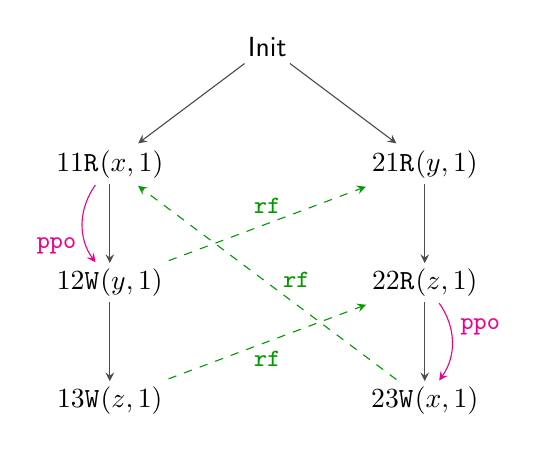
\begin{tikzpicture}[xscale=1,yscale=1.5]
  \node (init) at (2,  1)  {$\Init$};
  \node (i11)  at (0,  0)   {$\mese{1}{1}{} \rlab{}{x}{1}$};
  \node (i12)  at (0, -1)   {$\mese{1}{2}{} \wlab{}{y}{1}$};
  \node (i13)  at (0, -2)   {$\mese{1}{3}{} \wlab{}{z}{1}$};
  \node (i21)  at (4,  0)   {$\mese{2}{1}{} \rlab{}{y}{1}$};
  \node (i22)  at (4, -1)   {$\mese{2}{2}{} \rlab{}{z}{1}$};
  \node (i23)  at (4, -2)   {$\mese{2}{3}{} \wlab{}{x}{1}$};
  \draw[rf] (i13) edge node[below] {\small$\lRF$} (i22);
  \draw[rf] (i23) edge node[pos=.4,above] {\small\phantom{j}$\lRF$} (i11);
  \draw[rf] (i12) edge node[above] {\small$\lRF$} (i21);
  \draw[ppo,out=230,in=130] (i11) edge node[left ,pos=0.8] {\small$\lPPO$} (i12);
  \draw[ppo,out=310,in=50 ] (i22) edge node[right,pos=0.3] {\small$\lPPO$} (i23);
  \draw[po] (init) edge (i11);
  \draw[po] (init) edge (i21);
  \draw[po] (i11)  edge (i12);
  \draw[po] (i12)  edge (i13);
  \draw[po] (i21)  edge (i22);
  \draw[po] (i22)  edge (i23);
\end{tikzpicture}}$
\caption{Пример программы и соответствующий ей \IMM граф}
\label{fig:lb-sim-ex}
\end{figure}


\subsection{Обход графа \IMM}
\label{sec:imm-trav}

Определение обхода графа \IMM. Основные инварианты обхода.

\subsection{Отношение симуляции}
\label{sec:simrel}

Далее опишем отношение симуляции $\simrel$.
В целях ясности и простоты изложения, 
в данном разделе будет приведена упрощенная версия формального
определения этого отношения, которая опускает некоторые
технические детали. Полная версия отношения симуляции
может быть найдена в \coq репозитории. 

Отношение симуляции $\simrel(P, T, G, TC, S, X)$
устанавливает взаимосвязь между структурой событий $S$
и графом сценария исполнения $G$ с помощью
функции $\ea : S.\lE \fun G.\lE$, которая отображает
события структуры $S$ в события графа $G$.
Эта функция может быть натуральным образом
расширена на множества событий следующим образом%
\footnote{аналогично образом функций $\ea$ может быть расширена
на бинарные отношения на событиях.}:

\begin{align*}
\text{for } A_S \subseteq S.\lE        & :
  \fmap{A_S} \defeq \set{\ea(e) \in G.\lE \mid e \in A_S} \\
\text{for } A_G \subseteq G.\lE        & :
  \fcomap{A_G} \defeq \set{e \in S.\lE \mid \ea(e) \in A_G}.
\end{align*}

Отношение симуляции $\simrel(P, T, G, \TC, S, X)$ состоит из следующих свойств.

\begin{enumerate}

  \item \label{simrel:events}
    События $S$, принадлежащие потокам из $T$, а также события,
    принадлежащие конфигурации $X$, соответствуют покрытым событиям,
    а также выпущенным событиям и их $\lPO$-предшественникам: 
    \begin{itemize}
      \item $\fmap{S.\lE\rst{T}} = \fmap{X} = C \cup \dom{G.\lPO^? \seq [I]}$
    \end{itemize}

  \item \label{simrel:lab}
    Метки событий из $S$ совпадают с метками событий из $G$
    по модулю прочитанных или записанных значений. 
    \begin{enumerate}
      \setcounter{enumii}{0}
      \item \label{simrel:lab-eqmval}
        $\forall e \in S.\lE \ldotp\;
          S.\set{\lTID, \lTYP, \lLOC, \lMOD}(e) =
          G.\set{\lTID, \lTYP, \lLOC, \lMOD}(\fmap{e}) $
    \end{enumerate}
    Метки покрытых и выпущенных событий, принадлежащих конфигурации $X$,
    сопадают полностью.
    \begin{enumerate}
      \setcounter{enumii}{1}
      \item \label{simrel:lab-det}
        $\forall e \in X \cap \fcomap{C \cup I} \ldotp~
          S.\lVAL(e) = G.\lVAL(\ea(e))$
    \end{enumerate}

  \item \label{simrel:po}
    Программный порядок в структуре событий $S$
    совпадает с программным порядком в графе $G$:
    \begin{itemize}
      \item $\fmap{S.\lPO} \suq G.\lPO$
    \end{itemize}

  \item \label{simrel:cf}
    Если два события имеют одинаковый образ под действием функции $\ea$,
    то эти события равны или находятся в конфликте.
    \begin{itemize}
      \item $\fcomap{\mathtt{id}} \suq S.\lCF^?$
    \end{itemize}

  \item \label{simrel:jf}
    События чтения в $S$ должны быть обоснованы событиями записи,
    которые наблюдаются соответствующим событием чтением в $G$.
    \begin{enumerate}
      \item \label{simrel:jf-obs}
      \setcounter{enumii}{0}
        $\fmap{S.\lJF} \suq G.\lRF^?\seq G.\lHB^?$
    \end{enumerate}
    Более того, отношение $\lJF$, ограниченное на события чтения,
    принадлежащие конфигурации $X$, соответствуют
    отношению \emph{стабильной обоснованности} (\emph{stable justification})
    (смотри \cref{def:sjf}) в графе $G$.
    \begin{enumerate}
      \setcounter{enumii}{1}
      \item \label{simrel:jf-sjf}
        $\fmap{S.\lJF \seq [X]} \suq G.\lSRF_{TC}$
    \end{enumerate}
    %% As a consequence it is possible to derive that
    %% justification for covered events in $X$
    %% corresponds to their justification in $G$:
    %% $\fmap{S.\lJF \seq [X \cap \fcomap{C}]} \subseteq G.\lRF$. \\
    Только выпущенные события могут быть использованы для
    внешнего обоснования событий чтения. 
    \begin{enumerate}
      \setcounter{enumii}{2}
      \item \label{simrel:jfe-iss}
         $\dom{S.\lJFE} \suq \dom{S.\lEW \seq [X \cap \fcomap{I}]}$
    \end{enumerate}

  \item \label{simrel:ew}
    Все эквивалентные события записи в $S$ отображаются
    в одно и то же событие записи $G$.
    \begin{enumerate}
      \setcounter{enumii}{0}
      \item \label{simrel:ew-id}
        $\fmap{S.\lEW} \suq \mathtt{id}$
    \end{enumerate}
    Также каждый класс эквивалентности по отношению $S.\lEW^*$
    должен иметь представителя среди выпущенных событий,
    принадлежащих конфигурации $X$.
    \begin{enumerate}
      \setcounter{enumii}{1}
      \item \label{simrel:ew-iss}
        $S.\lEW \suq (S.\lEW \seq [X \cap \fcomap{I}] \seq S.\lEW)^?$
    \end{enumerate}

  \item \label{simrel:co}
    Если два события структуры $S$ находящихся в отношении когерентности,
    то их образы под действием функции либо также находятся
    в отношении когерентности, либо равны. 
    \begin{enumerate}
      \setcounter{enumii}{0}
      \item \label{simrel:co-co}
         $\fmap{S.\lCO} \suq G.\lCO^?$
    \end{enumerate}
    Если же ребро отношения когерентности оканчивается
    в событии, принадлежащем конфигурации $X$ и одному из потоков из $T$,
    тогда образ этого ребра принадлежит отношению когерентности в графе $G$.
    \begin{enumerate}
      \setcounter{enumii}{1}
      \item \label{simrel:co-cfg}
         $\fmap{S.\lCO \seq [X\rst{T}]} \suq G.\lCO$
    \end{enumerate}

  \item \label{simrel:sw-hb}
    Отношения ``синхронизируется-с'' и ``происходит-до''
    в структуре событий $S$ согласованы с соответствующими
    отношениями в графе $G$.
    \begin{enumerate}
      \item \label{simrel:sw}
        $\fmap{S.\lSW} \suq G.\lSW$
      \item \label{simrel:hb}
        $\fmap{S.\lHB} \suq G.\lHB$
    \end{enumerate}
\end{enumerate}

\begin{figure}[t]
$\hfill\inarr{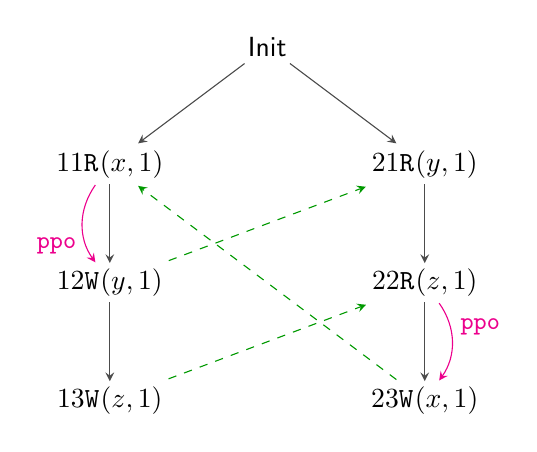
\begin{tikzpicture}[xscale=1,yscale=1.5]
  \node (init) at (2,  1)   {$\Init$};
  \node (i11)  at (0,  0)   {$\mese{1}{1}{} \rlab{}{x}{1}$};
  \node (i12)  at (0, -1)   {$\mese{1}{2}{} \wlab{}{y}{1}$};
  \node (i13)  at (0, -2)   {$\mese{1}{3}{} \wlab{}{z}{1}$};
  \node (i21)  at (4,  0)   {$\mese{2}{1}{} \rlab{}{y}{1}$};
  \node (i22)  at (4, -1)   {$\mese{2}{2}{} \rlab{}{z}{1}$};
  \node (i23)  at (4, -2)   {$\mese{2}{3}{} \wlab{}{x}{1}$};
  %% \node (hh)   at (2, -3.5) {$\inarrC{\text{The execution graph } G \text{ and} \\\text{its traversal configuration } \TCa}$};
  \begin{scope}[on background layer]
     \issuedCoveredBox{init};
     \issuedBox{i13};
%     \issuedBox{i23};
  \end{scope}
  \draw[rf] (i13) edge node[above] {} (i22);
  \draw[rf] (i23) edge node[above] {} (i11);
  \draw[rf] (i12) edge node[above] {} (i21);
% \draw[vf] (init) edge[bend right=20]  node[above left, pos=0.9] {$\lVF$} (i11);
% \draw[vf] (init) edge[bend left=20]  node[above right, pos=0.9] {$\lVF$} (i21);
% \draw[vf] (i13)  edge[bend right=20] node[above] {$\lVF$} (i22);
  \draw[ppo,out=230,in=130] (i11) edge node[left ,pos=0.8] {\small$\lPPO$} (i12);
  \draw[ppo,out=310,in=50 ] (i22) edge node[right,pos=0.3] {\small$\lPPO$} (i23);
  \draw[po] (init) edge (i11);
  \draw[po] (init) edge (i21);
  \draw[po] (i11)  edge (i12);
  \draw[po] (i12)  edge (i13);
  \draw[po] (i21)  edge (i22);
  \draw[po] (i22)  edge (i23);
\end{tikzpicture}}
\hfill\vrule\hfill
\inarr{\begin{tikzpicture}[scale=0.8, every node/.style={transform shape}]

  \node (init) at (0, 1)   {$\Init$};

  \node (i111) at (-1.5,  0)   {$\mese{1}{1}{1} \rlab{}{x}{0}$};
  \node (i121) at (-1.5, -1)   {$\mese{1}{2}{1} \wlab{}{y}{0}$};
  \node (i131) at (-1.5, -2)   {$\mese{1}{3}{1} \wlab{}{z}{1}$};

  \node (i211) at (0.5,  0)   {\phantom{$\mese{2}{1}{1} \rlab{}{y}{0}$}};
  \node (i221) at (0.5, -1)   {\phantom{$\mese{2}{2}{1} \rlab{}{z}{1}$}};
  \node (i231) at (0.5, -2)   {\phantom{$\mese{2}{3}{1} \wlab{}{x}{1}$}};

  \draw[jf] (init) edge[bend right] node[above]        {\small{$\lJF$}} (i111);

  \draw[po] (init)  edge (i111);
  \draw[po] (i111)  edge (i121);
  \draw[po] (i121)  edge (i131);

  \begin{scope}[on background layer]
    \draw[extractStyle] (-3, 1.5) rectangle (1,-2.5);
  \end{scope}

  %% \node (hh) at (0, -3.5) {$\inarrC{\text{The event structure } \ESa \text{ and} \\\text{the selected execution } \SXa}$};
\end{tikzpicture}}\hfill$
\caption{%
Граф сценария исполнения $G$, 
конфигурация его обхода $\TC_a$
и соответствующая этой конфигурации
структура событий $S_a$ вместе с конфигурацией $X_a$.
Покрытые события выделены как 
{\protect\tikz \protect\draw[coveredStyle] (0,0) rectangle ++(0.35,0.35);}
, а выпущенные как
{\protect\tikz \protect\draw[issuedStyle] (0,0) rectangle ++(0.35,0.35);}.
События, принадлежащие конфигурации $X_a$, выдены как 
{\protect\tikz \protect\draw[extractStyle] (0,0) rectangle ++(0.35,0.35);}.
}
\label{fig:lb-sim-ex-travA}
\end{figure}


\todo{пример}

\subsection{Шаг симуляции}
\label{sec:simstep}

В данном разделе приводится схема доказательства леммы \ref{lm:simstep}.
А именно, будет показано каким образом
операционная семантика построения структуры событий
симулирует шаг обхода графа \IMM.

Предположим, что для некоторых $P$, $G$, $\TC$, $S$ и $X$
выполняется отношение симуляции $\simrel(P, G, \TC, S, X)$.
Также положим, что в рамках обхода выполняется шаг
$G \vdash \TC \travstep{} \TC'$, который покрывает
или выпускает событие из потока с идентификатором $t$.
По условиям леммы \ref{lm:simstep} требуется предъявить
структуру $S'$ и конфигурацию $X'$,
такие что выполняется $\simrel(P, G, \TC', S', X')$.
Если поток $t$ содержит ещё непокрытые, но уже
выпущенные события записи, то необходимо выполнить
несколько шагов для построения из структуры $S$ структуры $S'$
чтобы добавить все события, $\lPO$-предшествующие непокрытым
событиям записи в потоке $t$.
Будем называть множество этих событий
\emph{сертификационной веткой},
а процесс добавление этих событий --- \emph{сертификацией}.

\begin{figure}[t]
$\hfill\inarr{\begin{tikzpicture}[xscale=1,yscale=1.5]
  \node (init) at (2,  1)   {$\Init$};
  \node (i11)  at (0,  0)   {$\mese{1}{1}{} \rlab{}{x}{1}$};
  \node (i12)  at (0, -1)   {$\mese{1}{2}{} \wlab{}{y}{1}$};
  \node (i13)  at (0, -2)   {$\mese{1}{3}{} \wlab{}{z}{1}$};
  \node (i21)  at (4,  0)   {$\mese{2}{1}{} \rlab{}{y}{1}$};
  \node (i22)  at (4, -1)   {$\mese{2}{2}{} \rlab{}{z}{1}$};
  \node (i23)  at (4, -2)   {$\mese{2}{3}{} \wlab{}{x}{1}$};
  %% \node (hh) at (2, -3.5) {$\inarrC{\text{The traversal configuration } \TCb}$};
  \begin{scope}[on background layer]
     \issuedCoveredBox{init};
     \issuedBox{i13};
     \issuedBox{i23};
  \end{scope}
  \draw[rf] (i13) edge node[above] {} (i22);
  \draw[rf] (i23) edge node[above] {} (i11);
  \draw[rf] (i12) edge node[above] {} (i21);
  \draw[vf] (init) edge[bend right=20]  node[above left, pos=0.9] {$\lVF$} (i11);
  \draw[vf] (init) edge[bend left=20]  node[above right, pos=0.9] {$\lVF$} (i21);
  \draw[vf] (i13)  edge[bend right=20] node[above] {$\lVF$} (i22);
  \draw[ppo,out=230,in=130] (i11) edge node[left ,pos=0.8] {\small$\lPPO$} (i12);
  \draw[ppo,out=310,in=50 ] (i22) edge node[right,pos=0.3] {\small$\lPPO$} (i23);
  \draw[po] (init) edge (i11);
  \draw[po] (init) edge (i21);
  \draw[po] (i11)  edge (i12);
  \draw[po] (i12)  edge (i13);
  \draw[po] (i21)  edge (i22);
  \draw[po] (i22)  edge (i23);
\end{tikzpicture}}
\hfill\vrule\hfill
\inarr{\begin{tikzpicture}[xscale=1,yscale=1.5]

  \node (init)  at (0, 1)      {$\Init$};

  \node (i111)  at (-1.5,  0)  {$\mese{1}{1}{1} \rlab{}{x}{0}$};
  \node (i121)  at (-1.5, -1)  {$\mese{1}{2}{1} \wlab{}{y}{0}$};
  \node (i131)  at (-1.5, -2)  {$\mese{1}{3}{1} \wlab{}{z}{1}$};

  \node (i211)  at (1.5,  0)   {$\mese{2}{1}{1} \rlab{}{y}{0}$};
  \node (i221)  at (1.5, -1)   {$\mese{2}{2}{1} \rlab{}{z}{1}$};
  \node (i231)  at (1.5, -2)   {$\mese{2}{3}{1} \wlab{}{x}{1}$};

  \draw[jf] (init) edge[bend right] node[above]        {\small{$\lJF$}} (i111);
  \draw[jf] (init) edge[bend left ] node[above]        {\small{$\lJF$}} (i211);
  \draw[jf] (i131) edge             node[pos=.5,below] {\small{$\lJF$}} (i221);

  \draw[po] (init)  edge (i111);
  \draw[po] (i111)  edge (i121);
  \draw[po] (i121)  edge (i131);

  \draw[po] (init)  edge (i211);
  \draw[po] (i211)  edge (i221);
  \draw[po] (i221)  edge (i231);

  \begin{scope}[on background layer]
    \draw[extractStyle] (-3, 1.5) rectangle (3,-2.5);
  \end{scope}

  %% \node (hh) at (0, -3.5) {$\inarrC{\text{The event structure } \ESb \text{ and} \\\text{the selected execution } \SXb}$};
\end{tikzpicture}}\hfill$
\caption{%
Граф сценария исполнения $G$, 
конфигурация его обхода $\TC_b$
и соответствующая этой конфигурации
структура событий $S_b$ вместе с конфигурацией $X_b$.
%% Покрытые события выделены как 
%% {\protect\tikz \protect\draw[coveredStyle] (0,0) rectangle ++(0.35,0.35);}
%% , а выпущенные как
%% {\protect\tikz \protect\draw[issuedStyle] (0,0) rectangle ++(0.35,0.35);}.
%% События, принадлежащие конфигурации $X_b$, выдены как 
%% {\protect\tikz \protect\draw[extractStyle] (0,0) rectangle ++(0.35,0.35);}.
}
\label{fig:lb-sim-ex-travB}
\end{figure}


Рассмотрим процесс построения сертификационной ветки
на примере шага обхода из конфигурации $\TC_a$ (\cref{fig:lb-sim-ex-travA})
в конфигурацию $\TC_b$ (\cref{fig:lb-sim-ex-travB})
путем выпуска события $\ese{2}{3}{}$.
Чтобы симулировать этот шаг, необходимо выполнить инструкции правого потока
и добавить в структуру событий ветку
$\Br_b = \set{\ese{2}{1}{1},\ese{2}{2}{1},\ese{2}{3}{1}}$
(смотри \cref{fig:lb-sim-ex-travB}).
Для того чтобы добавить эти события, в свою очередь,
выполняется построение трассы операционной семантики потока
${\state \thrdstep{\ese{2}{1}{1}}
         \thrdstep{\ese{2}{2}{1}}
         \thrdstep{\ese{2}{3}{1}}
         \state'}$, 
такой что
(i) она содержит все события правого потока
вплоть до последнего выпущенного события записи $\ese{2}{3}{}$ в графе $G$,
(ii) все эти события должны иметь тот же идентификатор потока,
тип обращения и локацию как и соответствующие события в графе
(то есть $\ese{2}{1}{}, \ese{2}{2}{}, \ese{2}{3}{}$),
(iii) все события, соответствующие покрытым и выпущенным событиям
(в данном случае~$\ese{2}{3}{1}$) должны иметь то же значение,
что и в графе $G$.
Для построения этой трассы используется свойство
\emph{восприимчивости} (\emph{receptiveness})
операционной семантики потока.
Это свойство позволяет выбрать произвольные значения
для всех промежуточных событий чтения в конструируемой трассе,
от которых не зависят (согласно отношению $\lDEPS$) выпущенные события записи%
\footnote{Формальное определение восприимчивости опущено
в данной работе для краткости и может быть найдено в \coq репозитории,
сопровождающем работу~\cite{Podkopaev-al:POPL19}.}.

Помимо этого, при добавлении новой ветки $\Br_b$ в структуру событий
необходимо выполнить следующие требования.
\begin{itemize}
  \item Для каждого события чтения (в данном случае $\ese{2}{1}{1}$ и $\ese{2}{2}{1}$)
    необходимо выбрать событие запись, обосновывающее это чтение.  
  \item Для каждого события записи необходимо определить позицию
    этого события в отношении частичного порядка $\lCO$.
\end{itemize}
Наконец, после завершения процесса сертификации,
новая ветка заменяет собой ветку потока $t$ в конфигурации $X$:
$$ X_b \defeq X_a \setminus S.\lE\rst{t} \cup \Br_b $$
где $S.\lE\rst{t} \defeq \set{e \in S.\lE \sth S.\lTID(e) = t}$.

\paragraph{Обоснование событий чтения.}

Далее рассмотрим процесс выбора обосновывающего события записи
для добавляемого события чтения.
Для этой цели определим отношение \emph{стабильной обоснованности}
в несколько этапов. 

Сначала по графу $G$ и текущей конфигурации обхода $\tup{C, I}$
зададим множество \emph{зафиксированных} (\emph{determined}) событий.
Метки зафиксированных событий а также события записи,
обосновывающие зафиксированные чтения, должны
совпадать в графе $G$, текущей структуре событий $S$,
а также в конструируемой сертификационной ветке $\Br$.

\begin{definition}
\label{def:det}
Множество \emph{зафиксированных событий}
определяется следующим соотношением.
\begin{align*}
  G.D_{\tup{C, I}} &\defeq {}
           C \cup I {}\cup{} \\
     %% &\cup G.\lW \setminus \codom{G.\lPPO} {}\cup{} \\
     &\cup \dom{G.\lRFI^? \seq G.\lPPO \seq [I]} {}\cup{} \\
     &\cup \cod{[I] \seq G.\lRFI} {}\cup{} \\
     &\cup \cod{G.\lRFE \seq [G.\lE^{\squq\acq}]}
\end{align*}
\end{definition}

Помимо покрытых и выпущенных событий
в множество зафиксированных событий также входят
все $\lPPO$-предшественники выпущенных событий,
все события чтения, читающие локально из некоторого выпущенного события,
а также события захватывающего ($\acq$) чтения,
читающие из другого потока. 

Для графа $G$ и конфигурации обхода $\TC_b$,
показанных на \cref{fig:lb-sim-ex-travB},
множество зафиксированных событий 
состоит из событий $\ese{1}{3}{}$, $\ese{2}{2}{}$ и $\ese{2}{3}{}$.
В то же время события $\ese{1}{1}{}$, $\ese{1}{2}{}$ и $\ese{2}{1}{}$
не являются зафиксированными, и следовательно
метки соответствующих им событий в структуре $S_b$
могут отличаться от меток в графе $G$.

Далее, введем понятие \emph{фронта} с помощью отношения $\lVF$.
Множество $\dom{\lVF \seq [e]}$ будем называть \emph{фронтом}
события $e$. Это множество содержит все события записи
``наблюдаемые'' событием $e$.
Будем говорить что $e$ \emph{наблюдает} событие записи $w$,
то есть $\tup{w, e} \in G.\lVF_{\TC}$, если
$w$ ``происходит-до'' $e$, либо оно было
прочитано некоторым покрытым событием, ``происходящим-до''~$e$,
либо оно было ранее прочитано некоторым зафиксированным событием
принадлежащем тому же потококу, что и~$e$. 

\begin{definition}
\label{def:vf}
Отношение $\lVF$ определено как:
\begin{align*}
  G.\lVF_{\tup{C,I}} \defeq {}
    [G.\lW] \seq (G.\lRF \seq [C])^? \seq G.\lHB^? \cup
    G.\lRF \seq [G.D_{\tup{C, I}}] \seq G.\lPO^?.
\end{align*}
\end{definition}

На \cref{fig:lb-sim-ex-travB} изображено три ребра отношения $G.\lVF_{\TC_b}$.
Все остальные ребра этого отношения могут быть выведены
при помощи следующего наблюдения:

$$ {G.\lVF_{\TC} \seq G.\lPO \subseteq G.\lVF_{\TC}}. $$

Наконец, можно привести определение отношения стабильной обоснованости.
Оно соединяет событие чтения с $\lCO$ максимальным
наблюдаемым событием записи в ту же локацию.

\begin{definition}
\label{def:sjf}
Отношение \emph{стабильной обоснованности} определяется следующим образом.
\begin{equation*}
  G.\lSRF_{TC} \defeq
    ([G.\lW] \seq (G.\lVF_{TC} \cap \lEQLOC) \seq [G.\lR])
    \setminus (G.\lCO \seq G.\lVF_{TC})
\end{equation*}
\end{definition}

Для графа $G$ и конфигурации $\TC_b$
отношение $\lSRF$ совпадает c показанными
на \cref{fig:lb-sim-ex-travB} ребрами отношения $\lVF$:
$$\tup{\Init, \ese{1}{1}{}}, \tup{\Init, \ese{2}{1}{}},
  \tup{\ese{1}{3}{}, \ese{2}{2}{}} \in G.\lSRF_{\TC_b}.$$

\begin{lemma}
\label{lm:sjf-det}
Если граф $G$ консистентен согласно модели \IMM,
тогда отношение $G.\lSRF$ совпадает с отношением $G.\lRF$
на множестве зафиксированных событий чтения.
$$  G.\lSRF_{\TC} ; [G.D_{\TC}] \subseteq G.\lRF $$
\end{lemma}

Лемма \ref{lm:sjf-det}, в частности, гарантирует, что
выбранные метки для событий чтения в сертификационной ветке,
от которых зависят (согласно отношению $\lDEPS$) выпущенные события записи,
будут согласованы с метками соответствующих событий в графе $G$.
Для всех остальных событий чтения, согласно свойству восприимчивости,
можно безопасно заменить прочитанные значения.

\begin{lemma}
\label{lm:sjf-iss-po}
Если граф $G$ консистентен согласно модели \IMM,
тогда для отношения $G.\lSRF$ выполняется следующие соотношение:
$$  G.\lSRF_{\TC} \suq [I] \seq G.\lSRF_{\TC} \cup G.\lPO. $$
\end{lemma}

Лемма \ref{lm:sjf-iss-po} позволяет выбрать обосновывающее
событие записи в структуре событий.
Пусть $\tup{w, r} \in G.\lSRF_{\TC}$.
Если при этом $\tup{w, r} \in [I] \seq G.\lSRF_{\TC}$
тогда, согласно свойству \ref{simrel:ew-iss} отношения симуляции
можно выбрать событие записи $w' \in S.\lE$, которое принадлежит
конфигурации $X$ и при этом соответствует выпущенной записи, то есть $\ea(w') = w$.
Например, в случае конфигурации обхода $\TC_b$, показанной на \cref{fig:lb-sim-ex-travB},
для события чтения $\ese{2}{2}{1}$
обосновывающим событием записи будет $\ese{2}{3}{1}$
Иначе $\tup{w, r} \in G.\lPO$.
В таком случае достаточно просто выбрать $S.\lPO$
предшествующее событие записи, принадлежащее сертификационной ветке $\Br$.

\paragraph{Упорядочивание событий записи.}

Позиция добавляемых событий записи в отношении порядка
$S.\lCO$ структуры событий выбирается на основе порядка
$G.\lCO$ \IMM графа. Тем не менее, из-за наличия конфликтующих событий,
можно гарантировать только лишь что отношение $S.\lCO$ вложено
в рефлексивное замыкание отношения $G.\lCO$,
то есть $\fmap{S.\lCO} \subseteq G.\lCO^?$.

\begin{figure}[t]
\hfill$\inarr{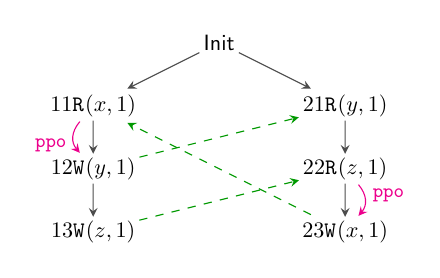
\begin{tikzpicture}[scale=0.8, every node/.style={transform shape}]
  \node (init) at (2,  1)   {$\Init$};
  \node (i11)  at (0,  0)   {$\mese{1}{1}{} \rlab{}{x}{1}$};
  \node (i12)  at (0, -1)   {$\mese{1}{2}{} \wlab{}{y}{1}$};
  \node (i13)  at (0, -2)   {$\mese{1}{3}{} \wlab{}{z}{1}$};
  \node (i21)  at (4,  0)   {$\mese{2}{1}{} \rlab{}{y}{1}$};
  \node (i22)  at (4, -1)   {$\mese{2}{2}{} \rlab{}{z}{1}$};
  \node (i23)  at (4, -2)   {$\mese{2}{3}{} \wlab{}{x}{1}$};
  %% \node (hh) at (2, -3) {$\inarrC{\text{The traversal configuration } \TCc}$};
  \begin{scope}[on background layer]
     \issuedCoveredBox{init};
     \issuedBox{i13};
     \issuedBox{i23};
     \coveredBox{i11};
  \end{scope}
  \draw[rf] (i13) edge node[above] {} (i22);
  \draw[rf] (i23) edge node[above] {} (i11);
  \draw[rf] (i12) edge node[above] {} (i21);
  %\draw[vf] (init) edge[bend left=20]  node[above right, pos=0.9] {$\lVF$} (i21);
  %\draw[vf] (i13)  edge[bend right=20] node[above] {$\lVF$} (i22);
  \draw[ppo,out=230,in=130] (i11) edge node[left ,pos=0.8] {\small$\lPPO$} (i12);
  \draw[ppo,out=310,in=50 ] (i22) edge node[right,pos=0.3] {\small$\lPPO$} (i23);
  \draw[po] (init) edge (i11);
  \draw[po] (init) edge (i21);
  \draw[po] (i11)  edge (i12);
  \draw[po] (i12)  edge (i13);
  \draw[po] (i21)  edge (i22);
  \draw[po] (i22)  edge (i23);
\end{tikzpicture}}
\hfill\vrule\hfill
\inarr{\begin{tikzpicture}[scale=0.8, every node/.style={transform shape}]
  \node (init) at (3, 1)     {$\Init$};

  \node (i111)  at (0,  0)   {$\mese{1}{1}{1} \rlab{}{x}{0}$};
  \node (i121)  at (0, -1)   {$\mese{1}{2}{1} \wlab{}{y}{0}$};
  \node (i131)  at (0, -2)   {$\mese{1}{3}{1} \wlab{}{z}{1}$};

  \node (i112)  at (3,  0)   {$\mese{1}{1}{2} \rlab{}{x}{1}$};
  \node (i122)  at (3, -1)   {$\mese{1}{2}{2} \wlab{}{y}{1}$};
  \node (i132)  at (3, -2)   {$\mese{1}{3}{2} \wlab{}{z}{1}$};

  \node (i211)  at (6,  0)   {$\mese{2}{1}{1} \rlab{}{y}{0}$};
  \node (i221)  at (6, -1)   {$\mese{2}{2}{1} \rlab{}{z}{1}$};
  \node (i231)  at (6, -2)   {$\mese{2}{3}{1} \wlab{}{x}{1}$};

  \draw[jf] (init) edge[bend right] node[above]        {} (i111);
  \draw[jf] (init) edge[bend left ] node[above]        {} (i211);
  \draw[jf] (i131) edge             node[pos=.5,below] {} (i221);
  \draw[jf] (i231) edge             node[pos=.5,below] {} (i112);

  \draw[cf] (i111) -- (i112);
  \node at ($.5*(i111) + .5*(i112) - (0, 0.2)$) {\small$\lCF$};

  \draw[co] (i122) edge node[pos=.5,below] {\small$\lCO$} (i121);
  \draw[ew] (i131) edge node[pos=.5,below] {\small$\lEW$} (i132);

  \draw[po] (init)  edge (i111);
  \draw[po] (i111)  edge (i121);
  \draw[po] (i121)  edge (i131);

  \draw[po] (init)  edge (i112);
  \draw[po] (i112)  edge (i122);
  \draw[po] (i122)  edge (i132);

  \draw[po] (init)  edge (i211);
  \draw[po] (i211)  edge (i221);
  \draw[po] (i221)  edge (i231);

  \begin{scope}[on background layer]
    \draw[extractStyle] (2, 1.5) rectangle (7,-2.5);
  \end{scope}

  %% \node (hh) at (3, -3.5) {$\inarrC{\text{The event structure } \ESc \text{ and} \\\text{the selected execution } \SXc}$};
\end{tikzpicture}}$\hfill
\caption{Граф сценария исполнения $G$, 
конфигурация его обхода $\TC_c$
и соответствующая этой конфигурации
структура событий $S_c$ вместе с конфигурацией $X_c$.
}
\label{fig:lb-sim-ex-travC}
\end{figure}


Данную особенность можно продемонстрировать 
на примере шага обхода из конфигурации $\TC_b$ (\cref{fig:lb-sim-ex-travB})
в конфигурацию $\TC_c$ (\cref{fig:lb-sim-ex-travC})
путем покрытия события $\ese{1}{1}{}$.
Для симуляции этого шага выполняется построение
структуры событий $S_c$, содержашей новую ветку 
$\Br_c \defeq \set{\ese{1}{1}{2}, \ese{1}{2}{2}, \ese{1}{3}{2}}$.

Рассмотрим события записи $\ese{1}{2}{1}$ и $\ese{1}{2}{2}$.
Так как два этих события имеют различные метки,
они не могут быть объявлены $\lEW$-эквивалентными.
С другой стороны, требуется, чтобы отношение
$S_c.\lCO$ полностью упорядочивало все события записи в одну и ту же локацию
(по модулю $\lEW$-эквивалентных событий).
То есть требуется каким-либо образом упорядочить
события $\ese{1}{2}{1}$ и $\ese{1}{2}{2}$ между собой.
Так как оба эти события отображаются в одно и то же событие $\ese{1}{2}{}$
в графе $G$, отношение $G.\lCO$ не может быть использовано
при выборе направления $S_c.\lCO$ ребра. 

На самом деле может быть выбран любой из двух способов
упорядочить эти события. Тем не менее,
в целях упрощения доказательства оказалось
удобнее выбрать порядок, при котором новые события
оказываются упорядочены ранее в отношении когеретности.
То есть, возвращаясь к примеру на \cref{fig:lb-sim-ex-travC},
стоит добавить ребро $\tup{\ese{1}{2}{2}, \ese{1}{2}{1}} \in S_c.\lCO$.
Используя данное соглашение можно показать, что
$S.\lCO$ ребро, оканчивающиеся событием из новой ветки $\Br_c$,
должно отображаться строго в ребро $G.\lCO$ в графе: 
$\fmap{S_c.\lCO \seq [\Br_c]} \suq G.\lCO$.

Далее рассмотрим события $\ese{1}{3}{1}$ и $\ese{1}{3}{2}$.
Эти события имеют одинаковую метку и отображаются в одно
и тоже событие $\ese{1}{3}{}$ в графе $G$.
Следовательно, они могут быть объявлены $\lEW$-эквивалентными.
На самом деле, для корректности построения их необходимо объявить таковыми.
Иначе события ветки $\Br_c$ окажутся невидимыми из-за того,
что существует путь $S_c.\lCF \cap (S_c.\lJFE \seq (S_c.\lPO \cup S_c.\lJF)^*)$
из события $\ese{1}{3}{1}$ в событие $\ese{1}{1}{2}$.
Напомним, что только видимые события могут быть использованы
для извлечения графа сценария исполнения из структуры событий
(смотри \cref{def:cfg}).

В общем случае, новое событие записи $e$
прикрепляется к классу эквивалентности по отношению $S.\lEW$,
представленному событием $w$, таким что
(i) $w$ имет тот же образ графе, что и $e$, то есть $\ea(w) = \ea(e)$;
(ii) $w$ принадлежит конфигурации $X$, а его образ в графе
принадлежит множеству выпущенных событий: $w \in X \cap \fcomap{I}$.
Если такого события $w$ не существует, тогда $e$
упорядочивается в отношении $S.\lCO$ до
множества событий, чьи образы в графе $G.\lCO$-предшествуют $\ea(e)$
и после событий, чьи образы в графе равны или $G.\lCO$-следуют за $\ea(e)$.
Благодаря свойству \ref{simrel:jfe-iss} отношения симуляции,
а именно $\dom{S.\lJFE} \suq \dom{S.\lEW \seq [X \cap \fcomap{I}]}$,
подобный выбор отношения $S'.\lEW$ гарантирует,
что все события из новой сертификационной ветки будут видимы. 

%% \specialsection{Выводы}
%% Жизнь --- тлен.
\pagebreak

\specialsection{Заключение}



\bibliographystyle{ugost2008}
\bibliography{main}

% Библиография в cpsconf стиле
% Аргумент {1} ниже включает переопределенный стиль с выравниванием слева
%% \begin{thebibliography}{1}
%% \bibitem{voc} Griffin D.W., Lim J.S. \flqq Multiband excitation vocoder\frqq. IEEE ASSP-36 (8), 1988, pp. 1223-1235.
%% \bibitem{vo2} Griffin D.W., Lim J.S. \flqq Multiband excitation vocoder\frqq. IEEE ASSP-36 (8), 1988, pp. 1223-1235.
%% \end{thebibliography}

\end{document}
